%% bare_conf.tex
%% V1.3
%% 2007/01/11
%% by Michael Shell
%% See:
%% http://www.michaelshell.org/
%% for current contact information.
%%
%% This is a skeleton file demonstrating the use of IEEEtran.cls
%% (requires IEEEtran.cls version 1.7 or later) with an IEEE conference paper.
%%
%% Support sites:
%% http://www.michaelshell.org/tex/ieeetran/
%% http://www.ctan.org/tex-archive/macros/latex/contrib/IEEEtran/
%% and
%% http://www.ieee.org/

%%*************************************************************************
%% Legal Notice:
%% This code is offered as-is without any warranty either expressed or
%% implied; without even the implied warranty of MERCHANTABILITY or
%% FITNESS FOR A PARTICULAR PURPOSE! 
%% User assumes all risk.
%% In no event shall IEEE or any contributor to this code be liable for
%% any damages or losses, including, but not limited to, incidental,
%% consequential, or any other damages, resulting from the use or misuse
%% of any information contained here.
%%
%% All comments are the opinions of their respective authors and are not
%% necessarily endorsed by the IEEE.
%%
%% This work is distributed under the LaTeX Project Public License (LPPL)
%% ( http://www.latex-project.org/ ) version 1.3, and may be freely used,
%% distributed and modified. A copy of the LPPL, version 1.3, is included
%% in the base LaTeX documentation of all distributions of LaTeX released
%% 2003/12/01 or later.
%% Retain all contribution notices and credits.
%% ** Modified files should be clearly indicated as such, including  **
%% ** renaming them and changing author support contact information. **
%%
%% File list of work: IEEEtran.cls, IEEEtran_HOWTO.pdf, bare_adv.tex,
%%                    bare_conf.tex, bare_jrnl.tex, bare_jrnl_compsoc.tex
%%*************************************************************************

% *** Authors should verify (and, if needed, correct) their LaTeX system  ***
% *** with the testflow diagnostic prior to trusting their LaTeX platform ***
% *** with production work. IEEE's font choices can trigger bugs that do  ***
% *** not appear when using other class files.                            ***
% The testflow support page is at:
% http://www.michaelshell.org/tex/testflow/



% Note that the a4paper option is mainly intended so that authors in
% countries using A4 can easily print to A4 and see how their papers will
% look in print - the typesetting of the document will not typically be
% affected with changes in paper size (but the bottom and side margins will).
% Use the testflow package mentioned above to verify correct handling of
% both paper sizes by the user's LaTeX system.
%
% Also note that the "draftcls" or "draftclsnofoot", not "draft", option
% should be used if it is desired that the figures are to be displayed in
% draft mode.
%
\documentclass[10pt, conference, compsocconf]{IEEEtran}
% Add the compsocconf option for Computer Society conferences.
%
% If IEEEtran.cls has not been installed into the LaTeX system files,
% manually specify the path to it like:
% \documentclass[conference]{../sty/IEEEtran}





% Some very useful LaTeX packages include:
% (uncomment the ones you want to load)


% *** MISC UTILITY PACKAGES ***
%
%\usepackage{ifpdf}
% Heiko Oberdiek's ifpdf.sty is very useful if you need conditional
% compilation based on whether the output is pdf or dvi.
% usage:
% \ifpdf
%   % pdf code
% \else
%   % dvi code
% \fi
% The latest version of ifpdf.sty can be obtained from:
% http://www.ctan.org/tex-archive/macros/latex/contrib/oberdiek/
% Also, note that IEEEtran.cls V1.7 and later provides a builtin
% \ifCLASSINFOpdf conditional that works the same way.
% When switching from latex to pdflatex and vice-versa, the compiler may
% have to be run twice to clear warning/error messages.






% *** CITATION PACKAGES ***
%
%\usepackage{cite}
% cite.sty was written by Donald Arseneau
% V1.6 and later of IEEEtran pre-defines the format of the cite.sty package
% \cite{} output to follow that of IEEE. Loading the cite package will
% result in citation numbers being automatically sorted and properly
% "compressed/ranged". e.g., [1], [9], [2], [7], [5], [6] without using
% cite.sty will become [1], [2], [5]--[7], [9] using cite.sty. cite.sty's
% \cite will automatically add leading space, if needed. Use cite.sty's
% noadjust option (cite.sty V3.8 and later) if you want to turn this off.
% cite.sty is already installed on most LaTeX systems. Be sure and use
% version 4.0 (2003-05-27) and later if using hyperref.sty. cite.sty does
% not currently provide for hyperlinked citations.
% The latest version can be obtained at:
% http://www.ctan.org/tex-archive/macros/latex/contrib/cite/
% The documentation is contained in the cite.sty file itself.






% *** GRAPHICS RELATED PACKAGES ***
%
\ifCLASSINFOpdf
% \usepackage[pdftex]{graphicx}
  % declare the path(s) where your graphic files are
  % \graphicspath{{../pdf/}{../jpeg/}}
  % and their extensions so you won't have to specify these with
  % every instance of \includegraphics
  % \DeclareGraphicsExtensions{.pdf,.jpeg,.png}
\else
  % or other class option (dvipsone, dvipdf, if not using dvips). graphicx
  % will default to the driver specified in the system graphics.cfg if no
  % driver is specified.
  % \usepackage[dvips]{graphicx}
  % declare the path(s) where your graphic files are
  % \graphicspath{{../eps/}}
  % and their extensions so you won't have to specify these with
  % every instance of \includegraphics
  % \DeclareGraphicsExtensions{.eps}
\fi
% graphicx was written by David Carlisle and Sebastian Rahtz. It is
% required if you want graphics, photos, etc. graphicx.sty is already
% installed on most LaTeX systems. The latest version and documentation can
% be obtained at: 
% http://www.ctan.org/tex-archive/macros/latex/required/graphics/
% Another good source of documentation is "Using Imported Graphics in
% LaTeX2e" by Keith Reckdahl which can be found as epslatex.ps or
% epslatex.pdf at: http://www.ctan.org/tex-archive/info/
%
% latex, and pdflatex in dvi mode, support graphics in encapsulated
% postscript (.eps) format. pdflatex in pdf mode supports graphics
% in .pdf, .jpeg, .png and .mps (metapost) formats. Users should ensure
% that all non-photo figures use a vector format (.eps, .pdf, .mps) and
% not a bitmapped formats (.jpeg, .png). IEEE frowns on bitmapped formats
% which can result in "jaggedy"/blurry rendering of lines and letters as
% well as large increases in file sizes.
%
% You can find documentation about the pdfTeX application at:
% http://www.tug.org/applications/pdftex





% *** MATH PACKAGES ***
%
%\usepackage[cmex10]{amsmath}
% A popular package from the American Mathematical Society that provides
% many useful and powerful commands for dealing with mathematics. If using
% it, be sure to load this package with the cmex10 option to ensure that
% only type 1 fonts will utilized at all point sizes. Without this option,
% it is possible that some math symbols, particularly those within
% footnotes, will be rendered in bitmap form which will result in a
% document that can not be IEEE Xplore compliant!
%
% Also, note that the amsmath package sets \interdisplaylinepenalty to 10000
% thus preventing page breaks from occurring within multiline equations. Use:
%\interdisplaylinepenalty=2500
% after loading amsmath to restore such page breaks as IEEEtran.cls normally
% does. amsmath.sty is already installed on most LaTeX systems. The latest
% version and documentation can be obtained at:
% http://www.ctan.org/tex-archive/macros/latex/required/amslatex/math/





% *** SPECIALIZED LIST PACKAGES ***
%
%\usepackage{algorithmic}
% algorithmic.sty was written by Peter Williams and Rogerio Brito.
% This package provides an algorithmic environment fo describing algorithms.
% You can use the algorithmic environment in-text or within a figure
% environment to provide for a floating algorithm. Do NOT use the algorithm
% floating environment provided by algorithm.sty (by the same authors) or
% algorithm2e.sty (by Christophe Fiorio) as IEEE does not use dedicated
% algorithm float types and packages that provide these will not provide
% correct IEEE style captions. The latest version and documentation of
% algorithmic.sty can be obtained at:
% http://www.ctan.org/tex-archive/macros/latex/contrib/algorithms/
% There is also a support site at:
% http://algorithms.berlios.de/index.html
% Also of interest may be the (relatively newer and more customizable)
% algorithmicx.sty package by Szasz Janos:
% http://www.ctan.org/tex-archive/macros/latex/contrib/algorithmicx/




% *** ALIGNMENT PACKAGES ***
%
%\usepackage{array}
% Frank Mittelbach's and David Carlisle's array.sty patches and improves
% the standard LaTeX2e array and tabular environments to provide better
% appearance and additional user controls. As the default LaTeX2e table
% generation code is lacking to the point of almost being broken with
% respect to the quality of the end results, all users are strongly
% advised to use an enhanced (at the very least that provided by array.sty)
% set of table tools. array.sty is already installed on most systems. The
% latest version and documentation can be obtained at:
% http://www.ctan.org/tex-archive/macros/latex/required/tools/


%\usepackage{mdwmath}
%\usepackage{mdwtab}
% Also highly recommended is Mark Wooding's extremely powerful MDW tools,
% especially mdwmath.sty and mdwtab.sty which are used to format equations
% and tables, respectively. The MDWtools set is already installed on most
% LaTeX systems. The lastest version and documentation is available at:
% http://www.ctan.org/tex-archive/macros/latex/contrib/mdwtools/


% IEEEtran contains the IEEEeqnarray family of commands that can be used to
% generate multiline equations as well as matrices, tables, etc., of high
% quality.


%\usepackage{eqparbox}
% Also of notable interest is Scott Pakin's eqparbox package for creating
% (automatically sized) equal width boxes - aka "natural width parboxes".
% Available at:
% http://www.ctan.org/tex-archive/macros/latex/contrib/eqparbox/





% *** SUBFIGURE PACKAGES ***
%\usepackage[tight,footnotesize]{subfigure}
% subfigure.sty was written by Steven Douglas Cochran. This package makes it
% easy to put subfigures in your figures. e.g., "Figure 1a and 1b". For IEEE
% work, it is a good idea to load it with the tight package option to reduce
% the amount of white space around the subfigures. subfigure.sty is already
% installed on most LaTeX systems. The latest version and documentation can
% be obtained at:
% http://www.ctan.org/tex-archive/obsolete/macros/latex/contrib/subfigure/
% subfigure.sty has been superceeded by subfig.sty.



%\usepackage[caption=false]{caption}
%\usepackage[font=footnotesize]{subfig}
% subfig.sty, also written by Steven Douglas Cochran, is the modern
% replacement for subfigure.sty. However, subfig.sty requires and
% automatically loads Axel Sommerfeldt's caption.sty which will override
% IEEEtran.cls handling of captions and this will result in nonIEEE style
% figure/table captions. To prevent this problem, be sure and preload
% caption.sty with its "caption=false" package option. This is will preserve
% IEEEtran.cls handing of captions. Version 1.3 (2005/06/28) and later 
% (recommended due to many improvements over 1.2) of subfig.sty supports
% the caption=false option directly:
%\usepackage[caption=false,font=footnotesize]{subfig}
%
% The latest version and documentation can be obtained at:
% http://www.ctan.org/tex-archive/macros/latex/contrib/subfig/
% The latest version and documentation of caption.sty can be obtained at:
% http://www.ctan.org/tex-archive/macros/latex/contrib/caption/




% *** FLOAT PACKAGES ***
%
%\usepackage{fixltx2e}
% fixltx2e, the successor to the earlier fix2col.sty, was written by
% Frank Mittelbach and David Carlisle. This package corrects a few problems
% in the LaTeX2e kernel, the most notable of which is that in current
% LaTeX2e releases, the ordering of single and double column floats is not
% guaranteed to be preserved. Thus, an unpatched LaTeX2e can allow a
% single column figure to be placed prior to an earlier double column
% figure. The latest version and documentation can be found at:
% http://www.ctan.org/tex-archive/macros/latex/base/



%\usepackage{stfloats}
% stfloats.sty was written by Sigitas Tolusis. This package gives LaTeX2e
% the ability to do double column floats at the bottom of the page as well
% as the top. (e.g., "\begin{figure*}[!b]" is not normally possible in
% LaTeX2e). It also provides a command:
%\fnbelowfloat
% to enable the placement of footnotes below bottom floats (the standard
% LaTeX2e kernel puts them above bottom floats). This is an invasive package
% which rewrites many portions of the LaTeX2e float routines. It may not work
% with other packages that modify the LaTeX2e float routines. The latest
% version and documentation can be obtained at:
% http://www.ctan.org/tex-archive/macros/latex/contrib/sttools/
% Documentation is contained in the stfloats.sty comments as well as in the
% presfull.pdf file. Do not use the stfloats baselinefloat ability as IEEE
% does not allow \baselineskip to stretch. Authors submitting work to the
% IEEE should note that IEEE rarely uses double column equations and
% that authors should try to avoid such use. Do not be tempted to use the
% cuted.sty or midfloat.sty packages (also by Sigitas Tolusis) as IEEE does
% not format its papers in such ways.





% *** PDF, URL AND HYPERLINK PACKAGES ***
%
%\usepackage{url}
% url.sty was written by Donald Arseneau. It provides better support for
% handling and breaking URLs. url.sty is already installed on most LaTeX
% systems. The latest version can be obtained at:
% http://www.ctan.org/tex-archive/macros/latex/contrib/misc/
% Read the url.sty source comments for usage information. Basically,
% \url{my_url_here}.





% *** Do not adjust lengths that control margins, column widths, etc. ***
% *** Do not use packages that alter fonts (such as pslatex).         ***
% There should be no need to do such things with IEEEtran.cls V1.6 and later.
% (Unless specifically asked to do so by the journal or conference you plan
% to submit to, of course. )


% correct bad hyphenation here
\hyphenation{op-tical net-works semi-conduc-tor}




% author names and affiliations
% use a multiple column layout for up to two different
% affiliations

\author{\IEEEauthorblockN{Yuji Mo and Stephen D. Scott}
\IEEEauthorblockA{Department of Computer Science\\
University of Nebraska\\
Lincoln, NE \ 68588-0115 USA\\
Email: \{ymo,sscott\}@cse.unl.edu}
%\and
% \IEEEauthorblockN{Stephen D. Scott}
% \IEEEauthorblockA{Department of Computer Science\\
% University of Nebraska\\
% Lincoln, NE \ 68588-0115 USA\\
% Email: sscott@cse.unl.edu}
\and
\IEEEauthorblockN{Doug Downey}
\IEEEauthorblockA{EECS Department\\
Northwestern University\\
Evanston, IL \ 60208 USA\\
Email: ddowney@eecs.northwestern.edu}
}


%\author{\IEEEauthorblockN{Authors Name/s per 1st Affiliation (Author)}
%\IEEEauthorblockA{line 1 (of Affiliation): dept. name of organization\\
%line 2: name of organization, acronyms acceptable\\
%line 3: City, Country\\
%line 4: Email: name@xyz.com}
%\and
%\IEEEauthorblockN{Authors Name/s per 2nd Affiliation (Author)}
%\IEEEauthorblockA{line 1 (of Affiliation): dept. name of organization\\
%line 2: name of organization, acronyms acceptable\\
%line 3: City, Country\\
%line 4: Email: name@xyz.com}
%}

% conference papers do not typically use \thanks and this command
% is locked out in conference mode. If really needed, such as for
% the acknowledgment of grants, issue a \IEEEoverridecommandlockouts
% after \documentclass

% for over three affiliations, or if they all won't fit within the width
% of the page, use this alternative format:
% 
%\author{\IEEEauthorblockN{Michael Shell\IEEEauthorrefmark{1},
%Homer Simpson\IEEEauthorrefmark{2},
%James Kirk\IEEEauthorrefmark{3}, 
%Montgomery Scott\IEEEauthorrefmark{3} and
%Eldon Tyrell\IEEEauthorrefmark{4}}
%\IEEEauthorblockA{\IEEEauthorrefmark{1}School of Electrical and Computer Engineering\\
%Georgia Institute of Technology,
%Atlanta, Georgia 30332--0250\\ Email: see http://www.michaelshell.org/contact.html}
%\IEEEauthorblockA{\IEEEauthorrefmark{2}Twentieth Century Fox, Springfield, USA\\
%Email: homer@thesimpsons.com}
%\IEEEauthorblockA{\IEEEauthorrefmark{3}Starfleet Academy, San Francisco, California 96678-2391\\
%Telephone: (800) 555--1212, Fax: (888) 555--1212}
%\IEEEauthorblockA{\IEEEauthorrefmark{4}Tyrell Inc., 123 Replicant Street, Los Angeles, California 90210--4321}}




% use for special paper notices
%\IEEEspecialpapernotice{(Invited Paper)}


%%%%%%%%%%%%%%%% old paper start here %%%%%%%%%%%%%%%% 

%\documentclass[twoside,leqno,twocolumn]{article}
% \documentclass[10pt,conference,compsocconf]{IEEEtran}
%\usepackage{ltexpprt} 
\usepackage{amsmath}
% % use Times
\usepackage{times}
% % For figures
\usepackage{graphicx} % more modern
% %\usepackage{epsfig} % less modern
\usepackage{subfigure} 
% % \usepackage{ulem} 
\usepackage{amssymb}
% % For citations
\usepackage[numbers,sort&compress]{natbib}
% 
% % For algorithms
\usepackage{algorithm}
\usepackage{algpseudocode}
\usepackage{hyperref}

\usepackage{color}

\definecolor{Red}{rgb}{1.0,0.0,0}
\definecolor{Blue}{rgb}{0.0,0.0,1}
\definecolor{Black}{rgb}{0.0,0.0,0.0}
\definecolor{Green}{rgb}{0.0,1.0,0.0}
\definecolor{Magenta}{rgb}{1.0,0.0,1}
\definecolor{Cyan}{rgb}{0.0,1.0,1}

\newcommand{\sys}{\Call{Hal}{}} % !!! WHEN YOU CHANGE THIS, YOU MUST MAKE A CORRESPONDING CHANGE IN 
% 				 %  TWO PLACES: where the term is defined in the text, and in the algorithm pseudocode.
% 
\newtheorem{thm}{Theorem}
\newtheorem{cor}{Corollary}[thm]
\newtheorem{prop}[thm]{Proposition}
\newtheorem{defn}[thm]{Definition}
\newtheorem{obs}[thm]{Observation}

% % correct bad hyphenation here
% \hyphenation{op-tical net-works semi-conduc-tor}

\begin{document}

% %
% % paper title
% % can use linebreaks \\ within to get better formatting as desired
\title{Learning Hierarchically Decomposable Concepts \\ with Active Over-Labeling}

% 
% % author names and affiliations
% % use a multiple column layout for up to three different
% % affiliations
% \author{\IEEEauthorblockN{Yuji Mo and Stephen D. Scott}
% \IEEEauthorblockA{Department of Computer Science\\
% University of Nebraska\\
% Lincoln, NE \ 68588-0115 USA\\
% Email: \{ymo,sscott\}@cse.unl.edu}
% %\and
% % \IEEEauthorblockN{Stephen D. Scott}
% % \IEEEauthorblockA{Department of Computer Science\\
% % University of Nebraska\\
% % Lincoln, NE \ 68588-0115 USA\\
% % Email: sscott@cse.unl.edu}
% \and
% \IEEEauthorblockN{Doug Downey}
% \IEEEauthorblockA{EECS Department\\
% Northwestern University\\
% Evanston, IL \ 60208 USA\\
% Email: ddowney@eecs.northwestern.edu}
% }

%\author{Yuji Mo\thanks{Dept. of Computer Science and Engineering, University of
%Nebraska, email: {\tt ymo@cse.unl.edu}}   \\
%\and
%Stephen Scott\thanks{Dept. of Computer Science and Engineering, University of Nebraska, email: {\tt sscott@cse.unl.edu}} 
%\and 
%Doug Downey\thanks{EECS Department, Northwestern University, email: {\tt ddowney@eecs.northwestern.edu}}
%}
%\date{}

%\maketitle



% make the title area
\maketitle



\begin{abstract} 
\begin{small}
%\baselineskip=9pt
Many classification tasks target high-level concepts
that can be decomposed into a hierarchy of finer-grained
subconcepts.  For example, some string entities that are Locations
are also Attractions, some Attractions are Museums, etc.  Such hierarchies are common in
named entity recognition (NER), document classification, and biological
sequence analysis.
We present a new approach for learning hierarchically decomposable
concepts.  The approach learns a high-level classifier
(e.g., location vs.\ non-location) by seperately learning multiple finer-grained
classifiers (e.g., museum vs.\ non-museum), and then combining the results.
Soliciting labels at a finer level of granularity
than that of the target concept is a new approach to active learning,
which we term {\em active over-labeling}.
In experiments in NER and document classification tasks, we show that active over-labeling substantially
improves area under the precision-recall curve
when compared with standard passive or active learning.
Finally, because finer-grained labels may be more expensive to obtain, we also present a cost-sensitive
active learner that uses a multi-armed bandit approach to dynamically choose the label granularity to target, and show that the 
bandit-based learner is
robust to differences in label cost and labeling budget.
\end{small}
\end{abstract} 

% \begin{keywords}
% Semi Supervised Learning, Active Learning, Hierarchical Labeling, Text Classification, Cost Analysis
% \end{keywords}

%\maketitle


\section{Introduction}
\label{sec:intro}
Several applications of machine learning have instances
that can be classified with hierarchical labeling
schemes.  For example, in named entity recognition (NER), the phrase
``The Metropolitan Museum of Art'' can be labeled as a Location, as a Building,
or as a Museum, where each label forms a subcategory of the
previous one.  Likewise, in the Gene Ontology (GO)~\cite{GeneOntology},
a biological sequence can be
labeled with multiple terms from a hierarchical scheme.

While some recent work has considered classification into fine-grained (low-level) 
categories \cite{fleischman2002fine,ling2012fine}
or hierarchies \cite{yosef2012hyena}, the majority of classification tasks in practice
target a small number of labels.  NER, for example, typically
targets a small set of coarse-grained labels such as Location, Organization,
and Person \cite{finkel2005incorporating}. 

We show how classifiers 
aimed at coarse-grained tasks can be improved by training on fine-grained labels.  For
example, we show that an NER system can be made more precise by not
treating the broad ``Organization'' label as a {\bf single} concept, but instead explicitly 
learning a combination of fine-graned labels comprising the category 
(e.g., ``University,'' ``Railroad Company,'' and so on).  As we argue theoretically 
in Section~\ref{sec:learningtheory} and establish in our experiments,
 % (e.g., see Figure \ref{fig:RPCurve-Whole}),
fine-grained labeling information can significantly improve the accuracy of a classifier aimed at a 
coarse-grained task.  Further, actively soliciting informative fine-grained labels, rather
than passively sampling them, provides an additional performance boost.  
We refer to this new approach, which extends the standard active
learning model to one in which the learner can solicit labels at finer
levels of the hierarchy than that targeted for classification,
as {\bf active over-labeling}.  

%In our work (Section~\ref{sec:results}), we discovered
%benefits to leveraging finer-grained label data (near the leaves
%of a label hierarchy) of instances to aid in building classifiers
%for coarse-grained labeling problems (near the root of a hierarchy).
%In our experiments, we discovered that one could leverage such fine-grained
%label data to improve precision for the same level of recall when 
%compared to learning algorithms that exclusively used coarse-grained
%labels.  

We present a general schema for performing active over-labeling
for any given hierarchical classification task, using
any given probabilistic base learner.  In our experiments, we demostrate
the effectiveness of the schema across multiple classification tasks (NER and document
classification) and multiple base learners (Conditional Random Fields and Logistic Regression).
We show that over-labeling improves performance over standard
passive or active learning, and that active over-labeling outperforms passive
over-labeling, in terms of area under the precision-recall curve.

Finally, we expect that obtaining a finer-grained
label will often be more costly than obtaining
a coarse-grained label.  For example, in GO, one could
label a sequence as being involved in biological processes, but a finer-grained
label for the same sequence could specify it as involved in growth,
% immune system process,
localization, or one of 22 other labels, which 
%.  The specificity of the fine-grained label 
requires more expertise and effort
to obtain.  Thus, we also present a method that uses a multi-armed bandit
approach to dynamically balance
cost and estimated benefit when choosing the level of granularity to
query.  We then show that the bandit approach is robust to changes in
label cost.

%We work in the {\it active learning} setting, where the labels of the training instances are initially unknown, 
%and a learning algorithm pays a certain cost to an oracle to reveal
%the labels of certain instances.  We study
%the cost/benefit trade-offs of making more expensive, fine-grained
%label purchases versus the less expensive coarse-grained purchases.

%In addition to our contribution of extending active learning to hierarchical labeling
%schemes, this paper contributes a new family of algorithms for over-labeling, 
%as well as an empirical cost/benefit analysis, determining 
%at what relative price points one would prefer one algorithm over another.

The rest of this paper is organized as follows.  In Section~\ref{sec:defn},
we define our learning setting and give intuition as to why
our approach offers advantages in this context.  
%Section \ref{sec:learningtheory} provides theoretical results showing
%that over-labeling improves computational complexity and label complexity
%when compared to conventional passive or active learning.
In Section~\ref{sec:approach} we describe
our algorithms in our new model, and we then present 
experimental results in Section~\ref{sec:results}.
%, where we discuss the benefit of using
%fine grained labels Section~\ref{sec:benefit}, our cost sensitivity analysis Section~\ref{sec:cost-sens}
%and empirical results on a self-adaptive learner Section~\ref{sec:adaptive}
We cover related work in Section~\ref{sec:relwork} and conclude in Section~\ref{sec:concl}.

\section{Problem Definition}
\label{sec:defn}

Our setting resembles conventional pool-based active learning.
Formally, our task is to learn a target concept over an input space ${\cal X}$,
i.e., a 
function $f : {\cal X} \rightarrow {\cal Y}=\{0, 1\}$.  We are given a pool of 
unlabeled examples $U \subset {\cal X}$, a base probabilistic machine learner $L$ that can
be trained on labeled examples $({\bf x}, y)$, and
access to an oracle that can be queried at some cost for the label of any example $u \in U$.
Our goal is to choose a relatively small number of examples from $U$ to be labeled, 
and train $L$ on the labeled examples to output a relatively accurate classifier.

Our setting resembles conventional active learning models in that the learner
purchases labels and builds its classifier in order to make predictions of the labels of new 
instances.  The key distinction is that in our model, the oracle can also return
more refined label information for each query example.  Specifically, we consider target
concepts that can be decomposed hierarchically into constituent subconcepts,
at varying levels of granularity.  We assume the decomposition is given
to the learner, and that the oracle can then return labels corresponding to any
node in the hierarchy, which we refer to as a {\bf labeling tree}.  An
example labeling tree based on Reuters Corpus Volume~I~(RCV1)~\cite{Lewis2004}
is shown in Figure~\ref{fig:ontologyex}.

Formally, nodes of the tree each represent concepts (i.e., subsets of the instance space ${\cal X}$).
The root of the labeling tree corresponds to the target concept to be learned, and lower 
levels of the tree are sub-concepts of their ancestor concepts.  The oracle in our
setting returns a {\it vector} of labels, corresponding to a path starting at the root of the tree.
For example, based on the label tree in
Figure~\ref{fig:ontologyex}, an instance could be labeled as
$\langle$Location,Building,Museum$\rangle$,  $\langle$Location,Attraction,Museum$\rangle$,
$\langle$Location,Lake,$X\rangle$, or $\langle X,X,X \rangle$, where an `$X$' indicates
that no value at that level applies.
Thus, the latter labeling example indicates an instance that is not a location.

\begin{figure}[ht]
\vskip 0.2in
\begin{center}
\centerline{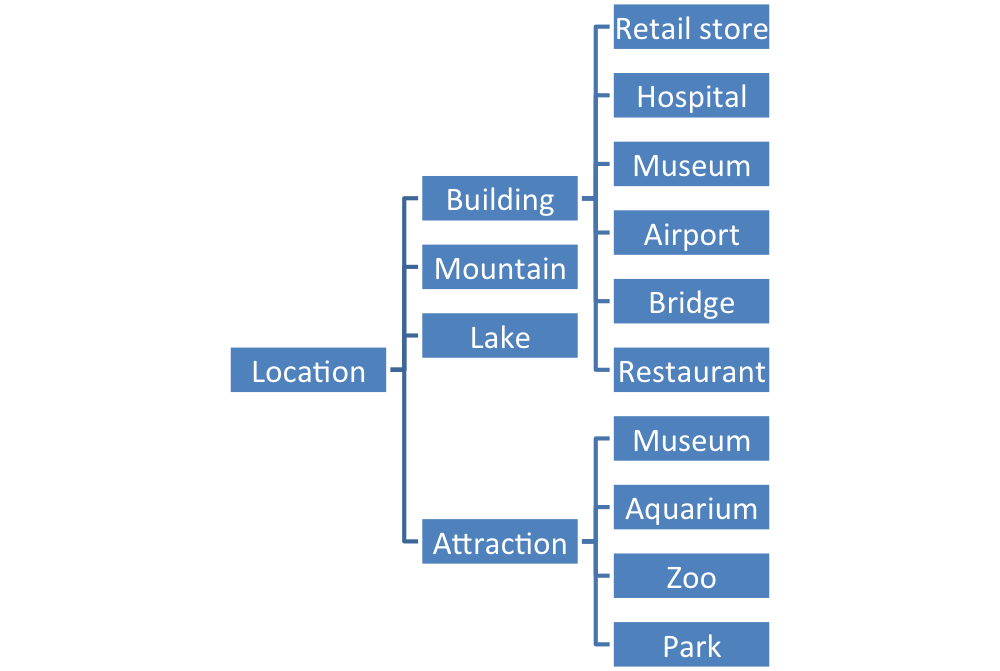
\includegraphics[width=1.1 \columnwidth]{fig/exp-ontology.png}}
\caption{An example labeling tree based on Reuters Corpus Volume~I~(RCV1)~\cite{Lewis2004}. 
}
\label{fig:ontologyex}
\end{center}
\vskip -0.2in
\end{figure} 

A vector of labels is denoted $\langle \ell_1,\ldots,\ell_k \rangle$, where a
label $\ell_i$ is the instance's label at the $i$th level of the tree, or `$X$' if that is
undefined in the tree.  If $\ell_i=X$, then $\ell_j=X$ for all $j > i$ (i.e., if a level-$i$
label does not apply, then no other label farther from the root may either).
Further, if $i$ is the largest value such that $\ell_i \neq X$, then
the values $\ell_i,\ldots,\ell_1$ must form a path from a leaf to the tree's root. 

Each instance in $U$ is initially labeled with the vector
$\langle$?,?,$\ldots$,?$\rangle$,
where `?' denotes a label value that is yet unspecified but can
be purchased.  For a specific instance, a value for $\ell_i$ may be purchased 
at cost $c_i \ge c_j > 0$ for all $i > j$.  We assume that a purchase of $\ell_i$ automatically
yields the values of $\ell_1$ through $\ell_{i-1}$.  E.g., a purchase of $\ell_3$ of an
instance could yield
$\langle$Location,Building,Museum$\rangle$,  $\langle$Location,Attraction,Museum$\rangle$,
$\langle$Location,Lake,$X\rangle$, or $\langle X,X,X \rangle$.\footnote{We assume that all labels in the
same level are distinct, e.g., `Museum' under `Attraction' is distinguishable from the one under
`Building'.}  %A minor change of notation would facilitate this, say, referring to the former as
%`Attraction-Museum' or `Location-Attraction-Museum'.}
Further, an $\ell_2$ purchase could yield
$\langle$Location,Building,?$\rangle$,  $\langle$Location,Attraction,?$\rangle$,
$\langle$Location,Lake,$X\rangle$, or $\langle X,X,X \rangle$ (once an `$X$' or a leaf
is encountered, one can fill in the rest of the vector with `$X$').

% commented by doug on 6/12, I think if we make the inequality non-strict we can 
% remove this sentence:
%We assume that $c_i \ge c_j > 0$ for all $i > j$ since otherwise there may be no incentive
%to purchase low-level labels.

%I'm not sure this adds enough to be included:
%Figure~\ref{fig:AL} illustrates the active learning model in a hierarchical labeling scheme.
%In this model, the active learning algorithm maintains one or more classifiers to predict labels
%for each level of the hierarchy.  Each iteration,
%the active learner considers the set of unlabeled data and chooses one or more unlabeled
%instances and a label level $i$ to purchase for those instances.  It then pays cost $c_i$ for 
%oracles to provide values of labels $\ell_1,\ldots,\ell_i$ for each such instance. 
%These labels and instances are then presented to learning algorithms to update classifiers 1
%through $i$.
%When learning is complete and a new instance $x$'s label is to be predicted, label
%predictions are made for $x$ by all classifiers at all levels, and these predictions are
%combined to make a final prediction for the root  level.  Final performance is based
%on how well predictions are made at the root level, and no others.

%\begin{figure}[ht]
%\vskip 0.2in
%\begin{center}
%\centerline{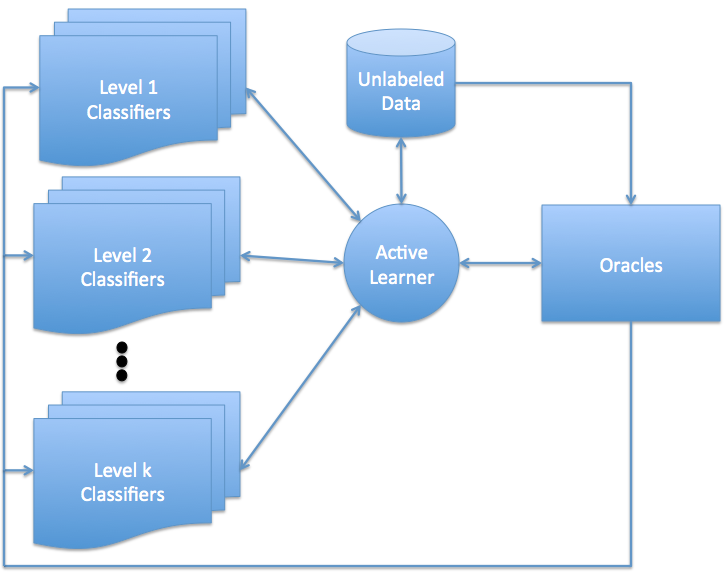
\includegraphics[width=\columnwidth]{fig/AL2.png}}
%\caption{The hierarchical active learning model.}
%\label{fig:AL}
%\end{center}
%\vskip -0.2in
%\end{figure} 


% Our work focuses on, based on the relative costs at each level,
% choosing at which levels to purchase labels.  


\subsection{Intuition}
\label{sec:intuition}

Over-labeling relies on learning classifiers for the fine-grained (non-root)
concepts and combining the results to predict the coarse-grained (root) label,
rather than simply directly learning the
coarse-grained (root) concept.  To see the potential advantage of over-labeling,
consider the simple example of
Figure~\ref{fig:unionex}.  In the figure, the coarse-grained concept
to be learned is circles (positives) versus diamonds (negatives).
If one limits the set of possible classifiers $\cal C$ to the set
of single axis-parallel boxes, then any hypothesis that has high recall
will have low precision (any rectangle that contains most of the circles will also
contain many diamonds).  However, if it is the case that the set
of positive instances can be decomposed into fine-grained classes
such as the four separate types of circles in Figure~\ref{fig:unionex},
then we can decompose the problem of classifying circles versus diamonds
into four problems: classifying green solid circles versus
everything else, classifying blue open circles versus everything
else, and so on.  We could thus train four fine-grained classifiers,
one per circle type.  With these inferred fine-grained classifiers,
one can predict on a new instance by predicting
its membership in each of the four fine-grained classes and then
returning a  root-level prediction of circle if any
fine-grained classifier predicts `yes'.  

In general, over-labeling takes advantage of a natural decomposition of the
target class into finer, possibly simpler sub-classes.  If the sub-classes
are in fact simpler to learn, then we can more easily learn the general class
by first learning the sub-classes and combining the sub-class predictions via, e.g., the 
union operator.  Since the union of hypotheses is a larger, more general
hypothesis space that includes the space of original hypotheses, this lends us
a potentially strong advantage in terms of representational ability.

\begin{figure}[ht]
\vskip 0.2in
\begin{center}
\centerline{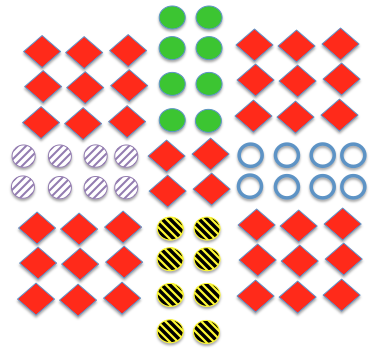
\includegraphics[width=2.in]{fig/union.png}}
\caption{ An example of the potential usefulness of learning multiple
fine-grained concepts to support
the learning of a single coarse-grained one.  Negative instances are diamonds and 
positive ones are circles. 
% Each size-8 cluster of circles represents a separate fine-grained concept.
}
\label{fig:unionex}
\end{center}
\vskip -0.2in
\end{figure} 

% Of course, real learning problems may not be as simple to decompose
% as that in Figure~\ref{fig:unionex}, but our experiments reveal
% clear empirical advantages.  

%Let's not mention cost here, we talked about this above.
%In general, we would anticipate that
%the fine-grained labels are more 
%expensive to obtain (e.g., when asked to label a phrase
%of text, a human labeler can probably distinguish the name of an
%attraction from that of a lake more easily than the
%name of a park from that of a zoo).  Thus, we how one can
%combine the use of labels at different labels to effectively learn
%the level-1 (root) concept.

\subsection{Learning-Theoretic Advantages}
\label{sec:learningtheory}

To formalize the intuitive advantage described in
Section~\ref{sec:intuition}, we present some simple theoretical
results that immediately follow from the literature.  This
section's purpose is not to advance the state of the art in 
learning theory, but to highlight the advantages that over-labeling
can provide.
We present observations in both the {\bf probably approximately correct
(PAC)}~\cite{v-tl-84} and {\bf exact}~\cite{a-lrsqc-87} models of learning. 
The results below focus on the 
% simple, but important 
case of learning concepts
that are unions of axis-parallel boxes 
% \textcolor{red}{(as in, e.g., decision trees \cite{})}
over real and  ordinal feature spaces.  
% Extending the results to other settings is an item of future work.

\subsubsection{PAC Learning with Active Over-labeling}
%\noindent {\bf 2.2.1 PAC Learning with Active Over-labeling}
In PAC, a learner is given parameters $0<\epsilon,\delta < 1/2$ 
and access to labeled training instances
drawn iid according to arbitrary distribution $\cal D$.  The
learner then outputs a hypothesis in polynomial time that,
with probability at least $1-\delta$, has error at most
$\epsilon$ on new instances drawn according to $\cal D$.  

\paragraph{Computational Complexity}
%\noindent {\bf 2.2.1.1 Computational Complexity}
% We begin by showing that in the passive learning setting, over-labeling
% offers advantages over standard labeling.
In the context  of computational complexity, we consider the case
% (in both the PAC and exact learning models)
of {\bf proper learning}\footnote{Note that the negative results described
below for both exact and PAC learning are only for proper learning.  One can
get positive results for these cases by allowing a logarithmic increase in the
number of boxes used, by applying the set cover approximation algorithm.},
in which the training instances are labeled by a
concept from $\cal C$ and the hypothesis inferred by the learner
is required to also be from $\cal C$.
%We consider the real space ${\cal X} = \mathbb{R}^d$.
%
%
We consider learning concepts  that are unions of
$k$ axis-parallel boxes in $\mathbb{R}^d$.  This
task is not properly PAC-learnable (i.e., learning $\cal C$ using $\cal C$)
if RP $\ne$ NP.
% a fact that can be obtained from results found in previous work.
\begin{obs}
The class of $k$-unions of axis-parallel boxes in $\mathbb{R}^d$ is not
properly PAC-learnable unless RP $=$ NP.
\end{obs}
{\bf Proof Sketch}: From Theorem 3.1.1 of Blumer et al.~\cite{behw-lvd-89}, 
concept class $\cal C$ is properly PAC learnable  iff there exists a 
randomized polynomial-time algorithm to find a hypothesis from $\cal C$
consistent with a sufficiently large labeled training sample 
$\cal X$ (called the {\bf consistent hypothesis problem}).
It is known to be NP-hard~\cite{behw-lvd-89,m-sncscp-xx} to find a smallest
set of rectangles to cover a set of points in $\mathbb{R}^d$ even
for $d=2$.  Thus, the consistent hypothesis problem for
$k$-unions of boxes is NP-hard, implying that one 
cannot properly PAC learn $k$-unions of boxes.  \hfill $\square$

In contrast, consider an over-labeling version of this learning problem,
% the $k$-unions of boxes problem,
in which each of the $k$ boxes
is a separate subconcept, as in Figure~\ref{fig:unionex}. 
Thus, examples from the $i$th box ($i=1,\ldots , k$) have a
fine-grained label (call it $I_i$) and all other 
examples are labeled `$-$'.
\begin{obs}
In the over-labeling setting, $k$-unions of boxes from $\mathbb{R}^d$
is properly PAC-learnable.
\end{obs}
{\bf Proof Sketch}: Let $m$ be the number of labeled training instances labeled
by the target concept of some $k$-union of boxes.
For each sub-concept, a consistent sub-hypothesis
(single bounding box)
can be learned from the fine-grained labels in time $O(dm)$.
The learner can learn each of the $k$ sub-concepts separately and
output their union in time $O(kdm)$, and this  union
will be consistent with all the labeled examples.
Thus, the consistent hypothesis problem can be solved in time polynomial in
$d$, $k$, and $m$.
Blumer et al.~\cite{behw-lvd-89} show that, if $m$ is sufficiently large,
then a consistent hypothesis $h$ will meet the PAC criteria.
Specifically, Equation~\ref{eqn:behw} below gives sufficient conditions on
$m$ for error bound $\epsilon$ and bound $\delta$ on probability of failure.
Because the over-labeling approach is finding a separate consistent hypothesis
for each of the $k$ fine-grained labels,
we apply Equation~\ref{eqn:behw}, but reduce
$\epsilon$ and $\delta$ each by a factor of $k$ to account for this.
This yields a polynomial bound on $m$.
% that is polynomial in all relevant parameters.
 \hfill $\square$

% \subsubsection{Sample Complexity}
% In the context of sample complexity, we look at passive PAC learning of unions of $k$
% axis-parallel boxes in $\mathbb{R}^d$.  The
% classic approach~\cite{behw-lvd-89} to PAC learning a function class $\cal C$ is to
% draw a labeled sample $\cal X$ of size  at least
% \begin{equation}
% m(\epsilon,\delta) = \max \left( {2 \over \epsilon} \log {2 \over \delta}, {8D \over \epsilon} \log {13
% \over \epsilon}  \right)
% \enspace ,
% \label{eqn:behw}
% \end{equation}
% where $\epsilon$ and $\delta$ are the PAC parameters and $D$ is
% the VC-dimension (VCD) of $\cal C$,
% and to then find some function $c \in {\cal C}$ consistent with
% $\cal X$.  
% 
% The VC-dimension of the class of single $d$-dimensional axis-aligned boxes is $2d$.  Based on
% Blumer et al.~\cite{behw-lvd-89}, then, the VCD of the $k$-union of
% $d$-dimensional axis-aligned boxes is
% $\Theta(d  k \log k)$.  Thus, to directly PAC-learn $k$-unions of $d$-dimensional boxes,
% it suffices to find a hypothesis consistent with 
% \[
% m_{coarse}(\epsilon,\delta) = \Theta \left( {1 \over \epsilon} \log {1 \over \delta}
% + {d k \log k \over \epsilon} \log {1 \over \epsilon}  \right)
% \enspace 
% \]
% labeled examples\footnote{Note that we are not considering the time complexity of finding such
% a consistent hypothesis, only the number of training instances.}.
% In contrast, learning the class of individual $d$-dimensional boxes reduces
% the VCD from $\Theta(d  k \log k)$ to $\Theta(d)$.  However, since the learning
% process is repeated $k$ times, one needs to learn each individual box with a smaller value of
% $\epsilon$ and a smaller value of $\delta$,
% to allow for the union bound to be applied across all $k$
% fine-grained hypotheses.  This yields a sample complexity of 
% \[
% m_{fine}(\epsilon/k,\delta/k) = \Theta \left( {k \over \epsilon} \log {k \over \delta}
% + {d k  \over \epsilon} \log {k \over \epsilon}  \right)
% \enspace 
% ,
% \]
% which grows more slowly than $m_{coarse}$.
% %  since  $m_{coarse}-m_{fine}$ is positive.

\paragraph{Label Complexity}
%\noindent {\bf 2.2.1.2 Label Complexity}
We now consider label complexity, in which one wants to minimize the 
number of labels purchased by a pool-based active learning algorithm.
We work in a model where we are given a size-$m$ set of training data $U$,
but initially the labels are missing. When seeking a PAC algorithm for learning, one
can apply a standard result from Blumer et al.~\cite{behw-lvd-89} that says if
the algorithm efficiently finds a hypothesis from $\cal C$ that is
consistent with $U$, which is
drawn iid from fixed distribution $\cal D$ and is of size at least
\begin{equation}
m(\epsilon,\delta) = \max \left( {2 \over \epsilon} \log {2 \over \delta}, {8D \over \epsilon} \log {13
\over \epsilon}  \right)
\label{eqn:behw}
\end{equation}
(where $D$ is the {\bf VC dimension} of ${\cal C}$),
then with probability $ \ge 1-\delta$, the hypothesis will have error
at most $\epsilon$.  If the instances of $U$ are 
unlabeled, the goal in active learning is to purchase as few as possible
labels of
instances of $U$ and still guarantee a hypothesis consistent with
all of $U$ (including the yet unlabeled ones), which would yield a PAC result. 

For this example, we focus on what we term the {\bf disjoint $k$-intervals
problem}.
% of learning axis-parallel boxes on the real line.
I.e., $\cal C$ is the set of unions of 
$ \le k$ disjoint intervals on $\mathbb{R}$. When a coarse-grained label
of instance $x \in U$ is purchased, it returns
`$+$' if $x$ lies in one of the $k$ target intervals and `$-$' otherwise.
When a fine-grained label of $x$ is purchased, the label is an indicator
of which of the $k$ target intervals it lies in ($I_1,\ldots,I_k$) or `$-$' if
it does not lie in any interval.  We assume that there is
at least one point from $U$ in each interval $I_j$ and that there is
at least  one point from $U$ between each adjacent pair of intervals.
% (otherwise, those empty intervals/gaps between intervals are irrelevant in the PAC sense).

In the following two observations, we 
bound the number of purchases needed in each labeling scheme to find a consistent
hypothesis.  Since the total number of instances needed for PAC learning
(per Equation~\ref{eqn:behw}) differs between them (due to different VC
dimensions), in the next two observations, we use $m_c$ for the 
number of instances in coarse-grained learning and $m_f$ needed
for fine-grained.

Assume that, for each target interval, there is
one instance of  $U$ that is pre-labeled for free.  I.e., in the 
coarse-grained case, there are $k$ instances labeled `$+$' (one in each target
interval) and in the fine-grained case there is one instance labeled $I_1$,
one labeled $I_2$, etc. 

\begin{obs}
The consistent hypothesis problem on disjoint $k$-intervals
with coarse-grained labels on $m_c$ instances requires
$\Omega(m_c)$ label purchases in the worst case.
\end{obs}
{\bf Proof Sketch}:  
The algorithm must find the
left and right boundaries of each of the $k$ target intervals, which
is tantamount to identifying the leftmost and rightmost negatively
labeled points between each consecutive pair of intervals.  Consider
two consecutive intervals $I_j$ and $I_\ell$. 
% that, when taken together and their intervening gap, contain the largest number of
% points from $U$ of all consecutive pairs of intervals.  Since
% it is the largest number of points, this count has to be $\Omega(m/k)$
% but could be $O(m)$ in the worst case.  
In searching for
the negative points from $U$ between $I_j$ and
$I_\ell$, the learner must purchase the label of some point between $x_j$ and
$x_\ell$, where $x_j$ and $x_\ell$ are the pre-labeled points from
$U$ from $I_j$ and $I_\ell$, respectively.
In the worst case, every query will result in a 
response of `$+$', until only one remains to be labeled
`$-$'.  Summed over all pairs of intervals, this 
requires $\Omega(m_c)$ purchases in the worst case. 
 \hfill $\square$

\begin{obs}
The consistent hypothesis problem on disjoint $k$-intervals
with fine-grained labels on $m_f$ instances
requires $O(k \log m_f)$ queries in the worst case.
\end{obs}
{\bf Proof Sketch}:  
An algorithm in the active over-labeling setting 
can perform a binary search between $x_j$ and $x_\ell$  (labeled
$I_j$ and $I_\ell$ rather than simply `$+$') until a negatively labeled
instance $x_-$ is found.  When
that is done, the learner can simply perform two binary searches: one between $x_-$ and
the right-most point in $I_j$ and one between $x_-$ and
the left-most point in $I_\ell$. This requires at most $O(\log m_f)$ queries
per pair of adjacent intervals, for a total of $O(k \log m_f)$ queries. 
 \hfill $\square$

% Thus, we see that active over-labeling requires exponentially fewer queries
% (in $m$) in the worst case when compared with standard active learning.

% classic approach~\cite{behw-lvd-89} to PAC learning a function class $\cal C$ is to
% draw a labeled sample $\cal X$ of size  at least
% \begin{equation}
% m(\epsilon,\delta) = \max \left( {2 \over \epsilon} \log {2 \over \delta}, {8D \over \epsilon} \log {13
% \over \epsilon}  \right)
% \enspace ,
% \label{eqn:behw}
% \end{equation}
% where $\epsilon$ and $\delta$ are the PAC parameters and $D$ is
% the VC-dimension (VCD) of $\cal C$,
% and to then find some function $c \in {\cal C}$ consistent with
% $\cal X$.  

To bound $m_c$, we use Equation~\ref{eqn:behw} with
VC dimension~\cite{behw-lvd-89} $D=2k$
and get (ignoring
the typically smaller first term) a number of purchases
$\Omega(m_c)= \Omega ((k / \epsilon ) (\log 1/\epsilon))$.
To bound $m_f$, note that we have $k$ independent learning problems, each a
single box.  Thus, we can use VC dimension~\cite{behw-lvd-89} $D=2$,
but the parameters $\epsilon$ and $\delta$
must each be reduced by a factor of $k$, since the errors of these hypotheses
accumulate.  Further, we must apply the learning process $k$ times, so (again
ignoring the first term) $m_f=O((k^2/\epsilon) \log (k/\epsilon))$, so 
our worst-case upper bound of purchases is
$O(k \log (k/\epsilon) + k \log \log (k/\epsilon))$. Both bounds grow linearly in $k$ but the
coarse-grained learner's bound is worse by a factor  exponential in $1/\epsilon$.

Simply put, the advantage that the fine-grained approach has comes from
the fact that, for positively-labeled instance $x \in U$, the fine-grained
label indicates the interval that $x$ lies in, while in the coarse-grained
approach, the label is simply `$+$'.  The distinct fine-grained label 
given by each interval allows for a binary search for interval boundaries,
hence the logarithmic dependence on $m_f$. In contrast,
the homogeneous `$+$' label across all intervals
for the coarse-grained labels can force a number of purchases linear in $m_c$.

% Finally, we can show that the worst-case number of label purchases required by a standard active learner
% is bounded above that of an active over-labeling learner.
% Applying Equation~\ref{eqn:behw},
% since the VC dimension $D$ of the union of $k$ intervals is $2k$, we will need
% $U$ of size 
% \[
% m \ge \max \left( {2 \over \epsilon} \log {2 \over \delta}, {16 k \over \epsilon} \log {13
% \over \epsilon}  \right)
% \enspace .
% \]
% The second term of the max is the dominant one (unless $\delta$ is exponentially small
% in $k$), so we focus on it.  This gives a worst-case lower bound 
% of purchases for a coarse-grained learner to be
% $\Omega ((k / \epsilon ) (\log 1/\epsilon))$,
% while our worst-case upper bound of purchases for a fine-grained learner is
% $O(k \log (k/\epsilon) + k \log \log (1/\epsilon))$. Both are linear in $k$ but the
% coarse-grained learner's bound is worse by a factor  exponential in $1/\epsilon$.

\subsubsection{Exact Learning with Active Over-Labeling}
%\noindent {\bf 2.2.2 Exact Learning with Active Over-Labeling}
We now illustrate the computational complexity advantages of
active over-labeling in the exact learning setting.  In 
exact learning, the learner gets access to two oracles: a
{\bf membership query} (MQ) oracle and an {\bf equivalence query}
(EQ) oracle.  An efficient learner will learn the exact identity
of the target concept in time and number of queries that are
polynomial in the problem size.  When the learner poses an EQ, it
passes to the oracle a hypothesis $h \in {\cal C}$ that it thinks is exactly
equivalent to the target concept, i.e., that will label all instances
correctly.  The oracle either responds that the hypothesis
is exactly correct or gives to the learner a counterexample, which
is an instance on which $h$ is wrong.  An MQ oracle receives from
the learner an instance $x$ and provides $x$'s label.  This is similar
to a pool-based active learning model, except that in the MQ model, the
instances can be arbitrary, while in pool-based active learning,
the instances must come from a pre-specified set.

We consider
%the passive (where all instances are labeled)
proper learning of $k$-unions of disjoint axis-parallel boxes,
in a bounded, discretized, $d$-dimensional instance space $\{0,\ldots,t-1\}^d$.
% (e.g., Figure~\ref{fig:unionex} using integer coordinates).

\begin{obs}
With over-labeling, disjoint $k$-unions of boxes 
% in a discrete space
can be exactly learned with
$O(k)$ EQs and $O(kd \log t)$ MQs and time polynomial in the number of queries.
\end{obs}
{\bf Proof Sketch}:
Using fine-grained labels for $k$ distinct fine-grained hypotheses (each using one 
box), one can exactly learn each box $j$ individually with one EQ (to get an
instance in box $j$)
and $O(d \log t)$ MQs (for binary search to find the box $j$'s $2d$
boundaries), for a
total of $O(k)$ EQs and $O(kd \log t)$ MQs and polynomial time.
%  polynomial in the number of queries.
 \hfill $\square$

This contrasts with a result from Bshouty and Burroughs~\cite{bb-plapc-03}
that one cannot exactly properly learn $k$-unions of axis-parallel boxes
when (constant) $d>2$ unless P $=$ NP.  I.e., while one 
can learn $k$-unions with $O(d \log k)$-unions, one cannot 
efficiently learn $k$-unions with $k$-unions  if P $\ne$ NP.  
%
Note that our positive result for over-labeling works for non-constant $d$, while the
hardness result for direct proper learning holds even for constant $d$. 
%Thus, there is clearly an advantage to having more refined label information in the form of which of the $k$ boxes an instance lies in.

% The above results show that in both the exact and PAC learning setting, and in active and passive learning,
% the over-labeling approach offers theoretical advantages over standard learning.  We now present
% our general method for active over-labeling, and evaluate it experimentally.


% \section{Theoretical Results}
% \label{sec:learningtheory}
% 
% We begin by proving formally that active over-labeling provides advantages
% in terms of both computational complexity and label complexity.  We present
% results in both the {\bf probably approximately correct
% (PAC)}~\cite{v-tl-84} and {\bf exact}~\cite{a-lrsqc-87} models of learning. 
% The results below focus on the simple, but important case of learning concepts
% that are unions of axes-parallel boxes 
% \textcolor{red}{(as in, e.g., decision trees \cite{})} over real
% or ordinal feature spaces.  Extending the results to other settings is an item
% of future work.
% 
% \subsection{PAC Learning with Active Over-labeling}
% 
% In the PAC model, a learner is given positive parameters $\epsilon,\delta < 1/2$ 
% and access to a set of labeled training instances
% drawn iid according to an arbitrary distribution $\cal D$.  The
% learner is then expected to output a hypothesis in polynomial time that,
% with probability at least $1-\delta$, has error at most
% $\epsilon$ on new instances drawn according to $\cal D$.  
% 
% \subsubsection{Computational Complexity}
% 
% We begin by showing that in the passive learning setting, over-labeling
% offers advantages over standard labeling.
% In the context  of computational complexity, we consider the case
% % (in both the PAC and exact learning models)
% of {\bf proper learning}, in which the training instances are labeled by a
% concept from $\cal C$ and the hypothesis inferred by the learner
% is required to also be from $\cal C$.
% %We consider the real space ${\cal X} = \mathbb{R}^d$.
% %
% %\footnote{Note that the negative results described below for both exact and PAC learning are only for proper learning.  One can get positive results for these cases by allowing a logarithmic increase in the number of boxes used, by applying the set cover approximation algorithm.
% %
% We consider the task of learning concepts that are unions of $k$ axes-parallel boxes in $\mathbb{R}^d$.  This
% task is not properly PAC-learnable if RP $\ne$ NP, a fact that can be obtained
% from results found in previous work.
% \begin{prop}
% Learning $k$-unions of axes-parallel boxes in $\mathbb{R}^d$ is not PAC-learnable unless RP $=$ NP.
% \end{prop}
% {\bf Proof}: From Blumer et al.~\cite{behw-lvd-89}, 
% a concept class $\cal C$ is properly PAC learnable  if and only if there exists a 
% polynomial-time algorithm to find a hypothesis from $\cal C$ consistent with a size-$m$ labeled training sample 
% $\cal X$ (this is called the {\bf consistent hypothesis problem}).
% It is known to be NP-hard~\cite{behw-lvd-89,m-sncscp-xx} to find a smallest
% set of rectangles to cover a set of points in $\mathbb{R}^d$ even
% for $d=2$.  Thus, the consistent hypothesis problem for
% $k$-unions of boxes is NP-hard, implying that one 
% cannot properly PAC learn $k$-unions of boxes.  \hfill $\square$
% 
% In contrast, consider an over-labeling version of this learning problem,
% % the $k$-unions of boxes problem,
% in which each of the $k$ boxes
% is a separate subconcept, as in Figure~\ref{fig:ontologyex}. 
% Thus, examples from the $i$th box ($i=1,\ldots , k$) have a
% fine-grained label (call it $I_j$) and all other 
% examples are labeled `$-$'.
% \begin{prop}
% In the over-labeling setting, $k$-unions of boxes is properly PAC-learnable.
% \end{prop}
% {\bf Proof}: For each subconcept, a consistent concept (a single bounding box) can be learned from the fine-grained labels in time $O(dm)$.
% Thus, the learner can learn each of the $k$ subconcepts separately and output their union in time $O(kdm)$, and this concept
% will be consistent with the labeled examples whenever such a concept exists.  Thus, here the consistent hypothesis
% problem can be solved in polynomial time, which Blumer et al.~\cite{behw-lvd-89} above 
% implies that $k$-unions with over-labeling is properly PAC learnable.
%  \hfill $\square$
% 
% % \subsubsection{Sample Complexity}
% % In the context of sample complexity, we look at passive PAC learning of unions of $k$
% % axis-parallel boxes in $\mathbb{R}^d$.  The
% % classic approach~\cite{behw-lvd-89} to PAC learning a function class $\cal C$ is to
% % draw a labeled sample $\cal X$ of size  at least
% % \begin{equation}
% % m(\epsilon,\delta) = \max \left( {2 \over \epsilon} \log {2 \over \delta}, {8D \over \epsilon} \log {13
% % \over \epsilon}  \right)
% % \enspace ,
% % \label{eqn:behw}
% % \end{equation}
% % where $\epsilon$ and $\delta$ are the PAC parameters and $D$ is
% % the VC-dimension (VCD) of $\cal C$,
% % and to then find some function $c \in {\cal C}$ consistent with
% % $\cal X$.  
% % 
% % The VC-dimension of the class of single $d$-dimensional axis-aligned boxes is $2d$.  Based on
% % Blumer et al.~\cite{behw-lvd-89}, then, the VCD of the $k$-union of
% % $d$-dimensional axis-aligned boxes is
% % $\Theta(d  k \log k)$.  Thus, to directly PAC-learn $k$-unions of $d$-dimensional boxes,
% % it suffices to find a hypothesis consistent with 
% % \[
% % m_{coarse}(\epsilon,\delta) = \Theta \left( {1 \over \epsilon} \log {1 \over \delta}
% % + {d k \log k \over \epsilon} \log {1 \over \epsilon}  \right)
% % \enspace 
% % \]
% % labeled examples\footnote{Note that we are not considering the time complexity of finding such
% % a consistent hypothesis, only the number of training instances.}.
% % In contrast, learning the class of individual $d$-dimensional boxes reduces
% % the VCD from $\Theta(d  k \log k)$ to $\Theta(d)$.  However, since the learning
% % process is repeated $k$ times, one needs to learn each individual box with a smaller value of
% % $\epsilon$ and a smaller value of $\delta$,
% % to allow for the union bound to be applied across all $k$
% % fine-grained hypotheses.  This yields a sample complexity of 
% % \[
% % m_{fine}(\epsilon/k,\delta/k) = \Theta \left( {k \over \epsilon} \log {k \over \delta}
% % + {d k  \over \epsilon} \log {k \over \epsilon}  \right)
% % \enspace 
% % ,
% % \]
% % which grows more slowly than $m_{coarse}$.
% % %  since  $m_{coarse}-m_{fine}$ is positive.
% 
% \subsubsection{Label Complexity}
% 
% We now consider label complexity, in which one wants to minimize the 
% number of labels purchased by a pool-based active learning algorithm.
% We will work in a model where we are given a size-$m$ set of training data $U$,
% but initially the labels are missing. When seeking a PAC algorithm for learning, one
% can apply a standard result from Blumer et al.~\cite{behw-lvd-89} that says if
% the algorithm efficiently finds a hypothesis consistent with $U$ with size at least
% \begin{equation}
% m(\epsilon,\delta) = \max \left( {2 \over \epsilon} \log {2 \over \delta}, {8D \over \epsilon} \log {13
% \over \epsilon}  \right)
% \label{eqn:behw}
% \end{equation}
% (where $D$ is the {\bf VC dimension} of ${\cal C}$),
% then with probability at least $1-\delta$, the hypothesis will have error
% at most $\epsilon$.  If the instances of $U$ are initially 
% unlabeled, the goal in active learning is to purchase as few labels of
% instances of $U$ as possible and still guarantee a consistent
% hypothesis to yield the PAC result. 
% 
% For this example, we focus on what we term the {\bf disjoint intervals
% problem}.
% % of learning axis-parallel boxes on the real line.
% That is, $\cal C$ is the set of unions of at
% most $k$ disjoint intervals on $\mathbb{R}$. When a coarse-grained label
% of instance $x \in U$ is purchased, it returns
% `$+$' if $x$ lies in one of the $k$ target intervals and `$-$' otherwise.
% When a fine-grained label of $x$ is purchased, the label is an indicator
% of which of the $k$ target intervals it lies in ($I_1,\ldots,I_k$) or `$-$' if
% it does not lie in any target interval.  We assume that there is
% at least one point from $U$ in each interval $I_j$ and that there is
% at least  one point from $U$ between each adjacent pair of intervals.
% % (otherwise, those empty intervals/gaps between intervals are irrelevant in the PAC sense).
% 
% We now analyze both the coarse-grained and fine-grained active learning
% models in this context. We assume that, for each target interval, there is
% one instance of  $\cal X$ that is pre-labeled (for free).  I.e., in the 
% coarse-grained case, there are $k$ instances labeled `$+$' (one in each target
% interval) and in the fine-grained case there is one instance labeled $I_1$,
% one labeled $I_2$, etc.
% 
% \begin{prop}
% The disjoint intervals problem with coarse-grained labels requires $\Omega(m)$ queries in the worst case.
% \end{prop}
% {\bf Proof}:  
% The goal of the algorithm is to find the
% left and right boundaries of each of the $k$ target intervals, which
% is tantamount to identifying the leftmost and rightmost negatively
% labeled points between each consecutive pair of intervals.  Consider
% two consecutive intervals $I_j$ and $I_\ell$. 
% % that, when taken together and their intervening gap, contain the largest number of
% % points from $U$ of all consecutive pairs of intervals.  Since
% % it is the largest number of points, this count has to be $\Omega(m/k)$
% % but could be $O(m)$ in the worst case.  
% In searching for
% the set of negative points from $U$ lying between $I_j$ and
% $I_\ell$, the learner must purchase the label of some point between $x_j$ and
% $x_\ell$, where $x_j$ and $x_\ell$ are the pre-labeled points from
% $U$ from $I_j$ and $I_\ell$, respectively (any other queries
% are superfluous).  In the worst case, every query will result in a 
% response of `$+$', until only one remains to be labeled
% `$-$'.  Summed over all adjacent pairs of intervals, this will
% require $\Omega(m)$ queries in the worst case. 
%  \hfill $\square$
% 
% \begin{prop}
% The disjoint intervals problem with fine-grained labels requires $O(k \log m)$
% queries in the worst case.
% \end{prop}
% {\bf Proof}:  
% An algorithm in the active over-labeling setting 
% can perform a binary search between $x_j$ and $x_\ell$  (labeled
% $I_j$ and $I_\ell$ rather than simply `$+$') until a negatively labeled
% instance $x_-$ is found.  When
% that is done, the learner can simply perform two binary searches: one between $x_-$ and
% the right-most point in $I_j$ and one between $x_-$ and
% the left-most point in $I_\ell$. This requires at most $O(\log m)$ queries
% per pair of adjacent intervals, for a total of $O(k \log m)$ queries. 
%  \hfill $\square$
% 
% Thus, we see that active over-labeling requires exponentially fewer queries
% (in $m$) in the worst case when compared with standard active learning.
% 
% % classic approach~\cite{behw-lvd-89} to PAC learning a function class $\cal C$ is to
% % draw a labeled sample $\cal X$ of size  at least
% % \begin{equation}
% % m(\epsilon,\delta) = \max \left( {2 \over \epsilon} \log {2 \over \delta}, {8D \over \epsilon} \log {13
% % \over \epsilon}  \right)
% % \enspace ,
% % \label{eqn:behw}
% % \end{equation}
% % where $\epsilon$ and $\delta$ are the PAC parameters and $D$ is
% % the VC-dimension (VCD) of $\cal C$,
% % and to then find some function $c \in {\cal C}$ consistent with
% % $\cal X$.  
% 
% Finally, we can show that the worst-case number of label purchases required by a standard active learner
% is bounded above that of an active over-labeling learner.
% Applying Equation~\ref{eqn:behw},
% Since the VC dimension $D$ of the union of $k$ intervals is $2k$, we will need
% $U$ of size 
% \[
% m \ge \max \left( {2 \over \epsilon} \log {2 \over \delta}, {16 k \over \epsilon} \log {13
% \over \epsilon}  \right)
% \enspace .
% \]
% The second term of the max is the dominant one (unless $\delta$ is exponentially small
% in $k$), so we focus on it.  This gives a worst-case lower bound 
% of purchases for a coarse-grained learner to be $\Omega ((k / \epsilon ) (\log 1/\epsilon))$,
% while our worst-case upper bound of purchases for a fine-grained learner is
% $O(k \log (k/\epsilon) + k \log \log (1/\epsilon))$. Both are linear in $k$ but the
% coarse-grained learner's bound is worse by a factor  exponential in $1/\epsilon$.
% 
% \subsection{Exact Learning with Active Over-labeling}
% 
% We illustrate the computational complexity advantages of
% active over-labeling in the exact learning setting.  In 
% exact learning, the learner gets access to two oracles: a
% {\bf membership query} (MQ) oracle and an {\bf equivalence query}
% (EQ) oracle.  An efficient learner will learn the exact identity
% of the target concept in time and number of queries that are
% polynomial in the problem size.  When the learner poses an EQ, it
% passes to the oracle a hypothesis $h$ that it thinks is exactly
% equivalent to the target concept, i.e., that will label all instances
% correctly.  The oracle either responds that the hypothesis
% is exactly correct or gives to the learner a counterexample, which
% is an instance on which $h$ is wrong.  An MQ oracle receives from
% the learner an instance $x$ and provides $x$'s label.  It is similar
% to an active learning model, except that in the MQ model, the
% instances can be arbitrary while in active learning, the instances must come
% from a pre-specified set.
% 
% Here we consider the passive (where all instances are labeled)
% proper learning of $k$-unions of axis-parallel boxes,
% in a bounded, discretized, $d$-dimensional instance space $\{0,\ldots,t-1\}^d$.
% 
% \begin{prop}
% With over-labeling, discrete $k$-unions of boxes can be exactly learned with
% $O(k)$ EQs and $O(kd \log t)$ MQs and time polynomial in the number of queries.
% \end{prop}
% {\bf Proof}:
% Using fine-grained labels for $k$ distinct fine-grained hypotheses (each using one 
% box), one can exactly learn each box individually with one EQ (to get a positive
% instance) and $O(d \log t)$ MQs (for binary search to find the box's $2d$ boundaries), for a
% total of $O(k)$ EQs and $O(kd \log t)$ MQs and time polynomial in the number of queries.
%  \hfill $\square$
% 
% This contrasts with a result from Bshouty and Burroughs~\cite{bb-plapc-03}
% that one cannot exactly properly learn unions of $\le k$ axis-parallel boxes
% ({\bf $k$-unions}) when (constant) $d>2$ unless P $=$ NP.  I.e., while one 
% can learn $k$-unions with $O(d \log k)$-unions, one cannot 
% efficiently learn $k$-unions with $k$-unions  if P $\ne$ NP.  
% %
% Note that the positive result for over-labeling works for non-constant $d$, while the
% hardness result for direct proper learning holds for constant $d$. 
% %Thus, there is clearly an advantage to having more refined label information in the form of which of the $k$ boxes an instance lies in.
% 
% The above results show that in both the exact and PAC learning setting, and in active and passive learning,
% the over-labeling approach offers theoretical advantages over standard learning.  We now present
% our general method for active over-labeling, and evaluate it experimentally.

\section{Approach}
\label{sec:approach}

We now present our method for performing the learning task outlined in 
Section~\ref{sec:defn}. 
We refer to our method as \sys, for Hierarchical Active Learner.
The high-level steps
of our algorithm are given in Algorithm~\ref{alg:treetrain}.  
%In
%our experiments, we explore variants of the basic algorithm,
%defined by 
%different strategies for purchasing labels and for assembling
%a coarse-grained level-1 classifier from the different classifiers
%learned for each level $i \le k$.  We describe the basic strategy
%and its variants below.

\sys\ iteratively purchases labels at each level of the labeling tree in batches,
where the proportion of labels purchased at each level is specified by
vector ${\bf p}$.  
% In our experiments, we explore how different settings for ${\bf p}$ impact performance. 
In the step \Call{Purchase}{$b \, p_i, i, C^*(x)$},
the system purchases $b \, p_i$ dollars worth of label vectors
defined up to level $i$ of the labeling tree, where the instances to be labeled are
chosen actively via uncertainty sampling relative to classifier\footnote{The {
\bf number} of examples purchased at each level will vary inversely with the cost of labels
at that level, and later we explore how varying label cost ratios impacts performance of the algorithm
for a given budget level.
% in our experiments
% (see Section~\ref{sec:cost-sens}).
} $C^*(x)$ (discussed below).
Because label vectors are defined up to level $i$, they include
labels for all levels $m \le i$ (Section~\ref{sec:defn}).
\Call{LabelMap}{$E', m, j$} then creates individual labeled examples for
class $m$ at level $j$
corresponding to the given label vectors $E'$, for training the classifiers $C_{i, j}$.

%After the level-$i$ purchase, the function \Call{LabelMap}{$E', m, j$} is called 
%for every level $m \le i$ and every class $j$ in level $m$.
%Calling \Call{LabelMap}{$E', m, j$} for each $j$ converts the purchased label vectors in 
%$E'$ into corresponding labels for level $m$
%Specifically, \Call{LabelMap}{}
%goes through every instance $x \in E'$ and $x$'s newly-purchased label vector $\langle \ell_1,
%\ldots, \ell_i,?,\ldots,? \rangle$, 
%and looks at the value $\ell_m$ of the level-$m$ label in
%the label vector.  
% Let the value of $\ell_m$ be $v$.  
%In the set $E_{m,j}$ returned by \Call{LabelMap}{$E', m, j$},
%instance $x$ is given a binary label of $1$ if $\ell_m=j$ and 0 otherwise.
%E.g., if $x$'s level-2 label is ``Lake'', then the label of $x$ in $E_{2,\mbox{Lake}}$ is
%1 and the label of $x$ in $E_{2,\mbox{Mountain}}$ is 0. 

%All examples purchased for level $j$ also serve
%as labeled examples for levels $i<j$, as discussed in the Section~\ref{sec:defn}.


%We experiment with two approaches for selecting which examples
%to label for level $i$.  The first ignores the classifier $C_{i,*}$ and simply
%selects examples at random---i.e.,
%it performs passive learning.  Our second approach uses active learning,
%selecting examples for level $i$ using {\it uncertainty sampling}~\cite{tk-svmalatc-01}
%relative to the current level-$i$ classifier \textcolor{magenta}{$C_{i,*}$} (discussed below).

\sys\ then trains a probabilistic binary classifier $C_{i,j}$ for each class $j$ 
at level $i$, using the machine learning algorithm $L$.  $C_{i,j}(x)$ denotes
$C_{i,j}$'s estimate of the probability that an arbitrary example $x$ is positive for class $j$ at level $i$ (e.g.,
$C_{2,\mbox{``Lake''}}(x)$ is the probability that instance $x$ is a Lake).  
The choice of $L$ depends on the particular learning task
(we use Gradient Boosted Regression Trees, Logistic Regression and Conditional Random Fields  in our experiments).

A key problem for \sys\ is how to combine the 
classifiers $C_{i,j}$ into an ensemble classifier for the coarse-grained level-1
concept.  In principle,
the level-1 concept is a disjunction over the concepts $j$ at any given level $i$.
However, modeling the $C_{i,j}$ for a given $i$ explicitly as a disjunction can be
challenging, due to dependencies across the different level-$i$ classifiers (which
are trained on related sets of data $E_{i,j}$).  
In preliminary experiments, we explored
combining the classifiers with a noisy-or model (i.e., assuming independence), a linear model~\cite{Breiman1996},
or taking a p-norm across all $j$.  None of these approaches outperformed a simple approach of
simply taking a maximum.  Thus, we define:
\begin{equation}
\label{eq:maxcombine}
%  C^*(x) = \left(\sum_{i,j}(C_{i,j}(x)^p) \right)^{1/p}
  C^*(x) = \max_{i,j} C_{i,j}(x)
\end{equation}
as the output ensemble classifier. 
%In our experiment, we choose $p=\infty$ so that Equation~\ref{eq:maxcombine} is equivalent to a maximum.

Finally, when purchasing examples with active learning, \sys\ uses uncertainty sampling.
The uncertainty at level $i$
is measured with respect to the ensemble classifier $C^*(x)$.  Specifically,
we define the uncertainty $u_i(x)$ of the label for example $x$ for level $i$ as:
\begin{equation}
 u(x) = 0.5 - | C^*(x) -0.5|
\enspace .
\end{equation}


\begin{algorithm}[ht]
\small{
\caption{Method for learning the concept at the root of labeling tree $T$.  
See text for 
Purchase and LabelMap.
% are separate subroutines (see text).
}
\label{alg:treetrain}
\begin{algorithmic}
\Function{Hal}{Unlabeled examples $U$, labeling tree $T$, machine learner $L$, budget
$B$, per-iteration budget $b$, Purchase proportions ${\bf p} = (p_1, \ldots , p_k)$ with
$||{\bf p}||_1=1$ and $p_i \ge 0$}
\State  $E_{i,j} \gets \emptyset$  \Comment binary-labeled train set for
level $i$, label $j$
\State Initialize $C_{i,j}$ for all $i, j$
\While{$B > b$}
  \State $B \gets B-b$
  \ForAll{Level $i \in T$}
    \State $E' \gets$ \Call{Purchase}{$b \, p_i, i, C_{i,*}$}
    \ForAll{Level $m \le i$}
       \ForAll{Class $j$ in Level $m$}
           \State $E_{m,j} \cup=$ \Call{LabelMap}{$E', m, j$} 
       \EndFor
    \EndFor
%    \Comment Purchase $b p_i$ labels for level $i$ (see text)
  \EndFor
  \ForAll{Level $i \in T$}
  \ForAll{Class $j$ in Level $i$}
    \State $C_{i,j} \gets$ Train $L$ on $E_{i,j}$
  \EndFor
  \EndFor
\EndWhile
\State \Return Ensemble classifier $C^*(\{C_{i,j}\}, {\bf p})$
%  \Comment Return an ensemble of the individual classifiers $C_i$ (see text)
\EndFunction
\end{algorithmic}
}
\end{algorithm}

\subsection{Dynamically Adapting Purchase Proportions}
\label{sec:adaptive}

\sys\ takes as input a vector of purchase proportions, specifying how much of the budget should be
spent acquiring labels at each given level of granularity in the hierarchy.  The cost of labeling an example can
vary across levels of the hierarchy, and as we show in Section~\ref{sec:cost-sens}, the relative benefit of labels from a given
level in the hierarchy often changes as learning progresses.  Thus, we desire a cost-sensitive approach that dynamically
adapts the purchase proportions.
% during learning.

We formulate the task of choosing which level of granularity to purchase next as a multi-armed bandit problem, and solve it using
Auer et al.'s~\cite{Auer2002} $\epsilon$-greedy bandit algorithm (we refer to
this approach as BANDIT).  For clarity, we focus on dynamically choosing
between two strategies corresponding to purchase proportions, ${\bf p}$ and ${\bf p'}$, but the generalization to more strategies is straightforward.

BANDIT iteratively chooses strategies, and uses a running average of the reward observed for each strategy to guide
its choices.  For active learning, a natural way to define reward in round $j$ is in terms of observed model change:
\begin{equation}
g_{j} = \frac{1}{\|X\|}\sum_{x_i \in X} \log{(|f_{j-1}(x_i) - f_{j}(x_i)|)}
\enspace ,
\end{equation}
where $X$ is the set of withheld {\em unlabeled} examples, and $f_{j}(x_i)$ is \sys's output for the 
input $x_i$ after the $j$th iteration.
% of \sys .

However, our problem setting has special characteristics that make the gain equation above unsuitable.
In particular, this gain score is not stationary as is assumed in the generic BANDIT
algorithm. Instead,
as the number of purchased examples increases and \sys\ gradually fits the data, the model becomes less likely to change. 
This means the running average of the gain will slowly decrease.  As a result,
BANDIT will disproportionately favor arms it has not played recently (whose average gains have not recently been updated).
In our preliminary experiments, we found that these characteristics led the generic BANDIT approach to thrash 
between arms in cases where sticking with one arm for longer was a stronger strategy.

To adapt BANDIT to our setting, instead of modeling each purchase strategy as
an arm, we instead use
two arms: (1) maintain the same strategy as before, and (2) switch strategies.
The reward from the first arm is always zero.  The reward from the second arm
depends on the difference in gain before and after switching, defined as:
\vspace{-0.1in}
\begin{equation}
\label{eq:reward}
    r_{j}=
\begin{cases}
   -\frac{g_{j}}{|g_{j}|}, & \text{if } {\bf p}\rightarrow{\bf p'}\\
    \frac{g_{j}}{|g_{j}|}, & \text{if } {\bf p'}\rightarrow{\bf p}\\
    0, & \text{if } {\bf p}\rightarrow{\bf p} \text{ or } {\bf p'}\rightarrow{\bf p'}\\
\end{cases}
\enspace .
\end{equation}
%We then utilize the average reward $r_j$ for a given arm within the existing 
%$\epsilon$-greedy bandit algorithm~\cite{Auer2002}.

\section{Experiments}
\label{sec:results}

We begin by describing the three datasets we will consider: a synthetic binary classification task,
and two real-world data sets in document classification and sequence tagging.
We then present our results.  We first show that active over-labeling
improves accuracy over standard active or passive learning. 
We then study how \sys 's 
performance varies with the relative labeling cost between
coarse (root) and fine (lower-level) labels and overall budget
(number of training examples).
Finally, we show how our adaptive bandit-based
over-labeling scheme, BANDIT, is robust
to changes in labeling cost and budget\footnote{The
code and dataset used in this experiment can be downloaded from
\url{http://github.com/moyuji/hal}}.

\subsection{Synthetic Dataset}
\label{sec:synth}

First we assess the advantage provided by using fine-grained label data in a synthetic binary
classification task. In this dataset the sole feature is a single continuous value
$x\in[0,18)$. The positive instances are all points in the $9$ level-3 intervals
$\{[0,1), [2,3), [4,5),\ldots,[16,17) \}$. We define the level-2 intervals by taking 
the union of consecutive triples of the level-3 intervals:
$\{[0,1), [2,3), [4,5) \}$, $\{[6,7), [8,9), [10,11) \}$, and
$\{[12,13), [14,15), [16,17) \}$. The level-1 label (positive versus negative) 
is the union of the three level-2 labels.
% (see~Figure~\ref{fig:hier-synth}). 
The goal is to learn the level-1 label of `$+$' versus `$-$'. 
We use as our base learner the Gradient Boosted Regression
Tree~(GBRT)~\cite{Friedman2001}, which is an ensemble of regression trees. 
We set the maximum depth in GBRT to be $1$ 
so that each tree maps to an interval. For the fine-grained learner,
the classifers at level 3 are combined with the level-2 classifier and then the
coarse-level classifier using Equation~\ref{eq:maxcombine}. Because GBRT can be
a union of intervals, the classifiers at each level should be expressive enough
to capture the target concept.


%%% SDS dropping this to save space
% \begin{figure}[h]
% \vskip 0.2in
% \begin{center}
% \centerline{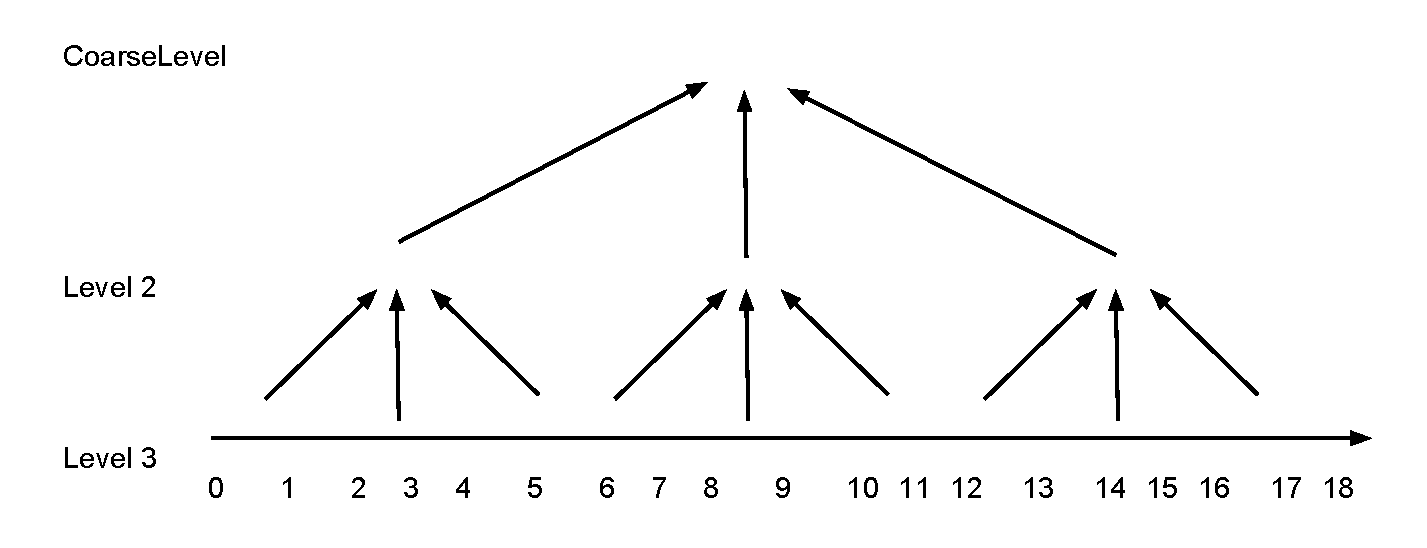
\includegraphics[width=\columnwidth]{fig/intervals.pdf}}
% \caption{The 3-level labeling  structure of the synthetic data set.}
% \label{fig:hier-synth}
% \end{center}
% \vskip -0.2in
% \end{figure} 

We chose $n=30$ trees, learning rate $\lambda=0.9$ and sample rate $r=0.8$ for our GBRT
learners.  Learners started with $100$ initial training
examples to ensure that all learners had initial instances in all fine-grained classes.
In each iteration, each learner purchases a label of  one instance from a pool of 10,000
instances.  We simulated noise by flipping the labels for 10\% of the examples
(choosing noisy fine-grained labels uniformly at random).
The classifiers are then tested against a set of 8,000 examples uniformly distriubuted in $[0,18)$.

\begin{figure}[tb]
	\centering
	\subfigure[Synthetic dataset]{
		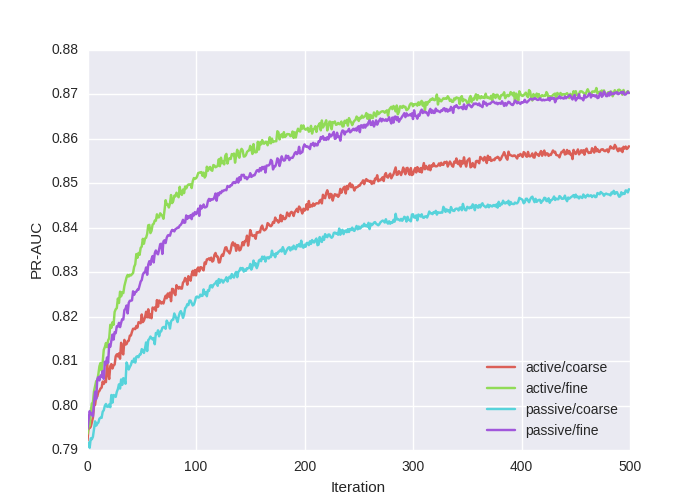
\includegraphics[width=\columnwidth]{fig/draft-interval}
		\label{fig:curve-synth}
	}\\
	\subfigure[Document classification]{
    	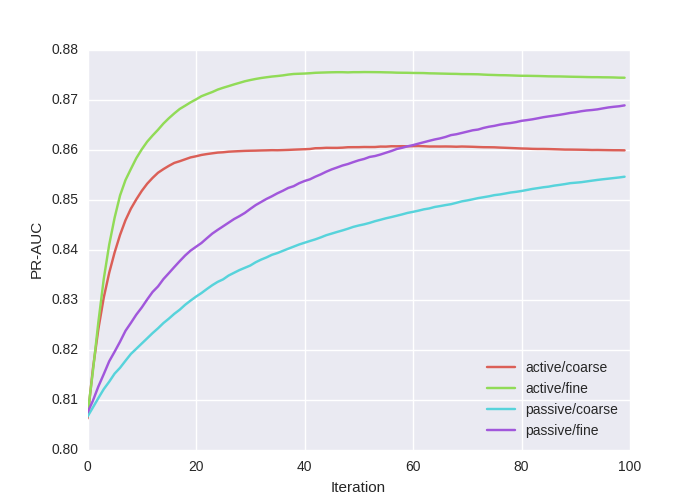
\includegraphics[width=\columnwidth]{fig/draft-RCV1}
    	\label{fig:curve-rcv1}
    }\\
    \subfigure[Sequence tagging]{
    	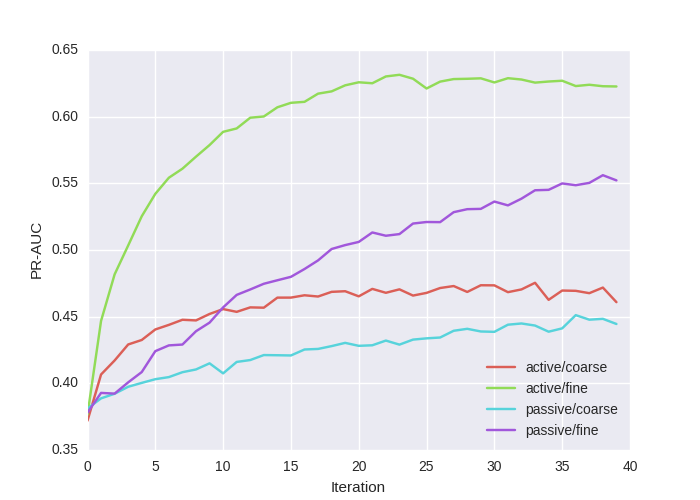
\includegraphics[width=\columnwidth]{fig/draft-richmond}
    	\label{fig:curve-richmond}
    }
    \caption{Learning curves comparing combinations of fine/coarse and active/passive PR-AUC}
  \label{fig:halresults}
\end{figure}

\subsection{Document Classification}
\label{sec:rcv1}

%We now present results from a document classification task.
The RCV1 data set~\cite{Lewis2004} contains 23,149 training documents and 781,265 test
documents labeled with a 117-node hierarchy  of Reuters Topics categories. 
Each document was represented in cosine-normalized log TF-IDF~\cite{Salton1988}
format.  Our coarse-based and fine-based learners used logistic regression~\cite{Cox1958} as
the base learner, with L2 regularization. (The regularization parameter of
$\lambda=0.1$ was chosen based on preliminary experiments; it is future work to
further tune this parameter via cross-validation.)

We used ECAT as the coarse-grained class, which contains 119,920
positive examples and 33 sub-classes in multiple levels underneath it.  
For this task we started with a seed set of 2,000 randomly-selected
instances and ran 100 iterations of active learning with 120 labels acquired
per iteration from the pool of the remaining 22,949 instances using both coarse-based and fine-based
methods. To eliminate trivially small classes,
we filtered out all fine-grained classes with fewer than 10 instances.
We tested the model on the entire test set, which is independent from the 
initial seed training set and candidate pool set. Each learning curve is the average of 50 rounds.

\subsection{Sequence Tagging}
\label{sec:richmond}

%Our third experiment focuses on entity recognition in sequences of text.  
We took OCR results from digitized editions of the {\it Richmond Daily
Dispatch} from November 1860 through December 1865 that had been
tagged with XML labels according to a two-level hierarchical labeling
scheme~\cite{RichmondDispatch}.  The dataset we used consists of
375,026 manually labelled organization names across 1,384 newspaper
articles.  These names are further categorized into a pool of 82
fine-grained categories, like bank names, railroad names and
government agency names.  Thus, the coarse-grained labels were
``organization'' versus ``not organization''
and each fine-grained label is, e.g., ``bank'' versus ``not bank''.

In the {\bf Dispatch} experiment, we used conditional random fields~(CRFs)~\cite{Sutton2006} 
as the base learner.  We trained CRFs using standard 2--3 letter prefix, postfix, capitalization and
numerical features.  We evaluate the trained CRF by performing 
the Forward-Backward algorithm~\cite{Culotta2004}
on a new sentence $s$ to get an estimate of the probability that each token
% (word or short phrase)
$x \in s$ is an organization.  Evaluating the set of tokens above
varying thresholds on this probability yields the precision-recall
curves we use for evaluation.

We compared training fine-based classifiers
via active learning, fine-based classifiers via passive learning,
coarse-based via active learning, and coarse-based via passive
learning.  First, we set aside 20,000 sentences for the test
set and 10,000 sentences for candidate set.
The experiment starts with a initial training set of 1,600 sentences.
For this task our experiments proceeded in 40 iterations, with batch sizes of
100 sentences each iteration. When computing the uncertainty of a sentence $s$,
we took the maximum uncertainty across all tokens in $s$.

\subsection{Results on active over-labeling}

For each of the three tasks described above, we built four learning curves.
The experiments compare four settings, for the four combinations of {\em active} vs. {\em passive}
learning,\footnote{Our passive learners
are trained with the same number of training instances as our active learners, but the
instances are chosen randomly rather than via uncertainty sampling.} and standard labeling vs. over-labeling with \sys .  Because standard learning
solicits coarse-grained labels for the coarse-grained task, we refer to that setting as {\em coarse}.
The coarse algorithms are representative of the state of the art in the document classification
and sequence tagging.  \sys\ uses finer-grained labels, so we refer to the over-labeling
setting as {\em fine}.

The results appear in Figure \ref{fig:halresults}.  As all three figures show, active over-labeling with
{\em active fine} is the best method across all three data sets.  These results show
how \sys\ improves accuracy by querying for examples at a finer granularity than 
that targeted for classification.

\subsection{Results as cost varies}
\label{sec:cost-sens}

The above results demonstrate the advantages offered by purchasing
fine-grained labels in an active learning context to improve performance.
So far, we have ignored differences in cost
between label types.  As discussed above, in practice fine-grained labels are likely to be
more expensive to obtain than coarse-grained labels, which means we might not be able to afford to
purchase purely fine-grained labels.

We first provide an analysis indicating that active over-labeling
is likely to provide value at varying ratios of cost between coarse and
fine-grained labels. We examine the learning curve of varying fixed ratio of
instances labeled at the fine and coarse levels in the experiments (FFR). For example,
in a setting of fine cost 16 and iteration budget of 32, FFR[0.5] allocates each of its 50\%
budget to coarse and fine, which corresponds to picking 16 coarse instances and 1 fine instance per iteration.
This curve will give us an estimate of what ratio of cost of fine-grained labels to coarse-grained
labels justifies the use of an active over-labeling approach.

\begin{figure}[tb]
	\centering
	\subfigure[Synthetic dataset]{
		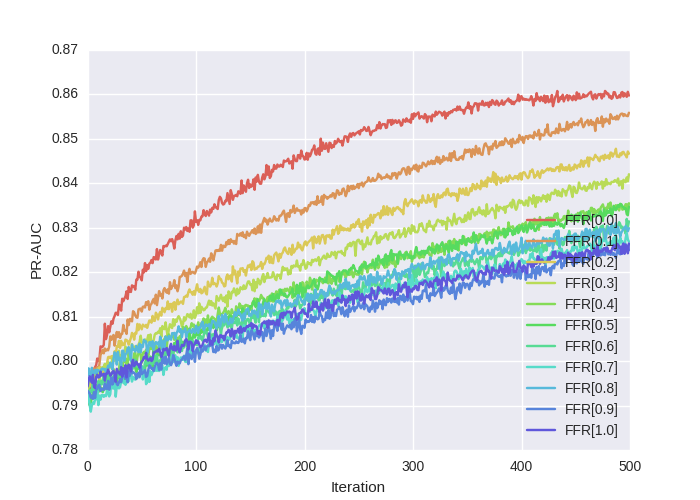
\includegraphics[width=\columnwidth]{fig/interval-16-nobandit}
		\label{fig:interval-cost16}
	}\\
	\subfigure[Document classification]{
    	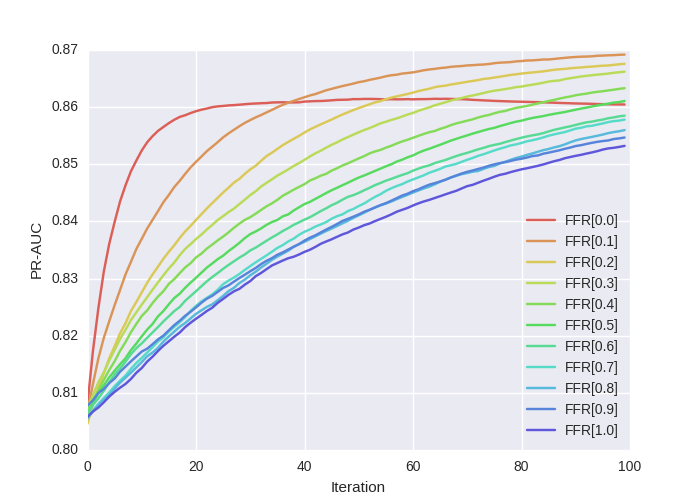
\includegraphics[width=\columnwidth]{fig/RCV1-16-nobandit}
    	\label{fig:RCV1-cost16}
    }\\
    \subfigure[Sequence tagging]{
    	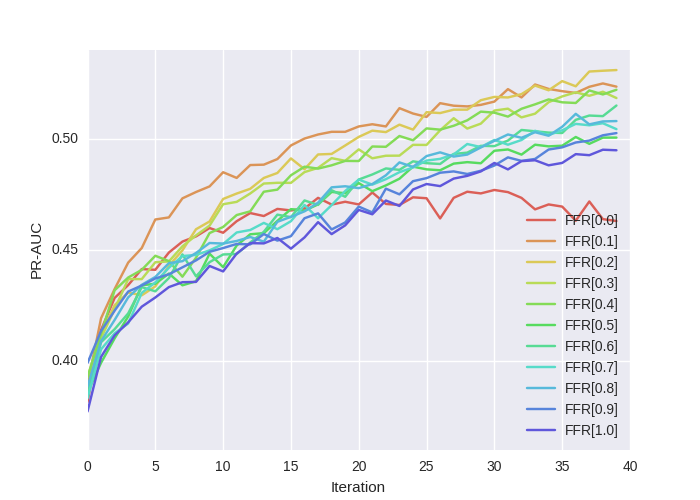
\includegraphics[width=\columnwidth]{fig/richmond-16-nobandit}
    	\label{fig:richmond-cost16}
    }
    \caption{Learning curves comparing active FFR method PR-AUC on fine cost 16}
	\label{fig:cost16}
\end{figure}

We switch from the fixed number of purchases per iteration to a fixed budget per iteration,
re-run the three experiments from Section~\ref{sec:synth}--Section~\ref{sec:richmond}, and then
compare the AUC scores achieved for active FFR learners in across experiments.

In Figure~\ref{fig:interval-cost16}, the synthetic dataset experiment, lower FFR
achieves better AUC in all $500$ iterations. The synthetic problem is easy to learn
which means the benefit of fine-grained labels cannot compensate for a fine cost as high as 16.
It is more cost effective to use a pure coarse-based classifier and not utilize fine-grained labels
at all.

In Figure~\ref{fig:RCV1-cost16}, the document classification experiment, FFR[0.0] rises fast
but quickly reaches a bottleneck, which is surpassed by FFR[0.1] in a later iteration. This problem
is less easy to learn and fine-grained labels may be worth their cost, depending on the overall budget.
If the budget is limited to fewer than 38 rounds, FFR[0.0] is the best choice; otherwise,
FFR[0.1] delivers better value than FFR[0.0].

\clearpage

In Figure~\ref{fig:richmond-cost16}, the sequence tagging experiment, the problem is harder,
so FFR[0.1]
has higher AUC than FFR[0.0] starting from the beginning. Then FFR[0.2] catches up after round 35. Higher FFR ratio
is more affordable in the long run. If the budget is less than 35 rounds then FFR[0.1] is preferred over FFR[0.2].

From Figure~\ref{fig:cost16}, we can see that the choice of FFR to achieve high AUC depends on multiple factors,
like the overall budget (the number rounds of iterations before termination), the cost of fine-grained labels and
the nature of the problem target itself.

\subsection{Results with BANDIT}

We now turn to evaluating BANDIT, which chooses purchase proportions dynamically.  We configure the two strategies
that BANDIT selects between to be the all-coarse (FFR[0.0]) and all-fine (FFR[1.0]) strategies.
We again set aside 20,000, 4,000 and 10,000 unlabeled examples for the synthetic task, document classification, 
and sequence tagging, and re-run the experiment in Section~\ref{sec:cost-sens} with
BANDIT. To evaluate the robustness of the algorithm, we test each approach for fine-grain cost varying within 
$\{1.0, 1.1, 1.2, 1.5, 2.0, 4.0, 8.0, 16.0, 32.0, 64.0\}$.


\begin{figure}[tb]
	\centering
	\subfigure[Synthetic dataset experiment]{
		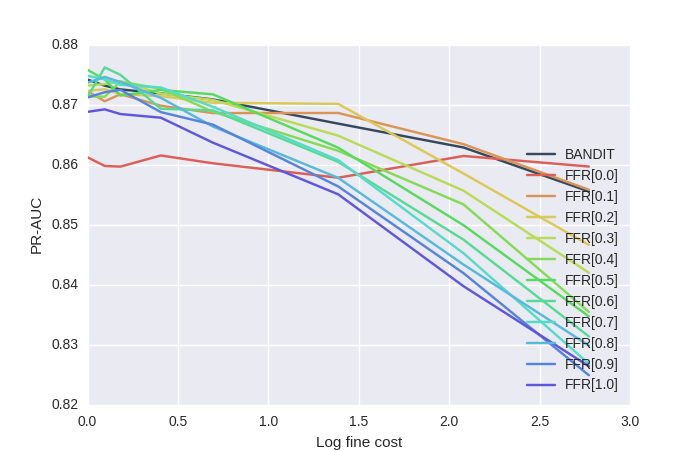
\includegraphics[width=\columnwidth]{fig/curve-interval}
		\label{fig:interval-curve}
	}\\
	\subfigure[Document classification experiment]{
    	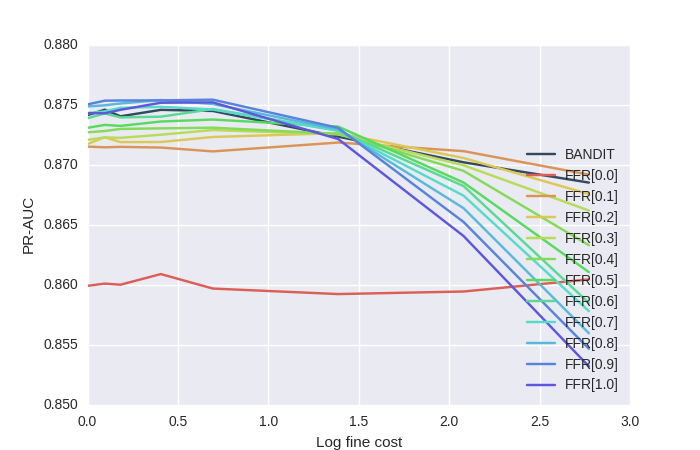
\includegraphics[width=\columnwidth]{fig/curve-RCV1}
    	\label{fig:RCV1-curve}
    }\\
    \subfigure[Sequence tagging experiment]{
    	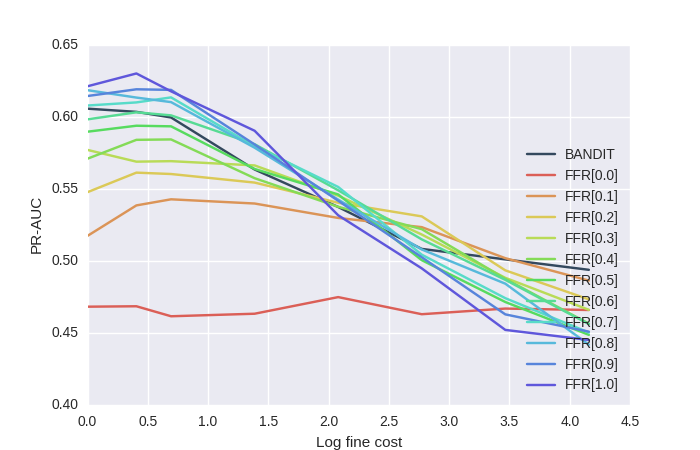
\includegraphics[width=\columnwidth]{fig/curve-richmond}
    	\label{fig:richmond-curve}
    }
    \caption{Comparing active FFR and BANDIT method PR-AUC on different fine cost}
	\label{fig:curve}
\end{figure}

Figure~\ref{fig:curve} shows the AUC for FFR and BANDIT in the end. We see that AUC in 
FFR[0.0] is not affected by the fine cost. And the AUCs for the other fixed ratio methods
FFR[0.1]-FFR[1.0] decrease as fine grained labels become more expensive, because that results in these methods 
acquiring fewer labels.
FFR with a lower fine-grained ratio achieves higher AUC when fine cost is high, and vice vesa. But the BANDIT curve is almost
always among the top curves, regardless of the fine cost. This shows how BANDIT is robust to changes in cost.

Tables~\ref{tb:synth}--\ref{tb:richmond} quantify
the observations in Figure~\ref{fig:curve}, by measuring
how close each learner is to the top-scoring learner as fine cost varies. 
The metric {\em diff} gives the learner's absolute difference from the top learner. The {\em rank} metric is
the learner's relative rank ordered by AUC.  We caculate the minimum, maximum, mean and standard deviation
for both metrics. In Table~\ref{tb:synth}, the diff of BANDIT is in the range of [0.001, 0.004] and averages
0.002 away from the top curve. and the rank of BANDIT ranges from 1 to 5 and averages 2.625.
BANDIT's mean for diff and rank is the lowest among all learners, and it has a low standard deviation, indicating
that BANDIT scores close to the top curve most of the time. 
Similar results are shown in Table~\ref{tb:RCV1} and Table~\ref{tb:richmond}, where the mean
diff of BANDIT is the lowest and the mean rank is the second lowest (as highlighted). These results illustrate
that BANDIT successfully tunes the fine-grained ratio  to cope with variable cost/benefit settings,
which is important in real-world settings where the costs and benefits from querying at different levels of granualrity
are not known in advance.

Finally, we examine how BANDIT performs as budget changes. Figure~\ref{fig:costmixed} shows the learning curves
of how AUC increases for FFR and BANDIT, averaging over different costs. On different tasks, different fine-grained
ratios may be preferable for different budgets---e.g., FFR[0.0] performs best for the first few purchases in Figure~\ref{fig:RCV1-costmixed}, but
is much worse for larger budgets.  However, in all figures, BANDIT almost always maintains the top AUC score
after the first few rounds. Thus, we expect BANDIT to perform well against fixed ratio methods across a variety of budgets.

\begin{table}[htb]
\caption{Aggregated PR AUC for synthetic dataset}
\centering
\resizebox{0.9\columnwidth}{!}{%
\begin{tabular}{lrrrrrrrr}
\hline
{} &  diff &       &       &       & rank &     &        &       \\
{} &   min &   max &  mean &   std &  min & max &   mean &   std \\
\hline
algorithm &       &       &       &       &      &     &        &       \\
BANDIT    & 0.001 & 0.004 & \underline{\textbf{0.002}} & 0.001 &    1 &   5 &  \underline{\textbf{2.625}} & 1.598 \\
FFR[0.0]  & 0.000 & 0.016 & 0.010 & 0.006 &    0 &  11 &  8.125 & 4.549 \\
FFR[0.1]  & 0.000 & 0.006 & 0.003 & 0.002 &    0 &   9 &  4.875 & 3.603 \\
FFR[0.2]  & 0.000 & 0.013 & 0.004 & 0.004 &    0 &   7 &  4.000 & 2.204 \\
FFR[0.3]  & 0.001 & 0.018 & 0.005 & 0.006 &    1 &   4 &  3.250 & 1.165 \\
FFR[0.4]  & 0.000 & 0.024 & 0.007 & 0.008 &    1 &   8 &  4.875 & 2.357 \\
FFR[0.5]  & 0.000 & 0.025 & 0.006 & 0.009 &    0 &   9 &  3.750 & 3.151 \\
FFR[0.6]  & 0.000 & 0.028 & 0.008 & 0.010 &    0 &   8 &  5.250 & 3.370 \\
FFR[0.7]  & 0.000 & 0.033 & 0.008 & 0.012 &    0 &   9 &  4.250 & 3.240 \\
FFR[0.8]  & 0.001 & 0.030 & 0.009 & 0.011 &    1 &   9 &  6.000 & 3.251 \\
FFR[0.9]  & 0.002 & 0.035 & 0.011 & 0.012 &    6 &  11 &  8.750 & 1.669 \\
FFR[1.0]  & 0.005 & 0.033 & 0.013 & 0.010 &   10 &  11 & 10.250 & 0.463 \\
\hline
\end{tabular}}
\label{tb:synth}
\end{table}

\begin{table}[htb]
\caption{Aggregated PR AUC for document classification}
\centering
\resizebox{0.9\columnwidth}{!}{%
\begin{tabular}{lrrrrrrrr}
\hline
{} &  diff &       &       &       & rank &     &        &       \\
{} &   min &   max &  mean &   std &  min & max &   mean &   std \\
\hline
algorithm &       &       &       &       &      &     &        &       \\
BANDIT    & 0.001 & 0.001 & \underline{\textbf{0.001}} & 0.000 &    1 &   8 &  3.750 & 2.188 \\
FFR[0.0]  & 0.009 & 0.016 & 0.014 & 0.002 &    6 &  11 & 10.375 & 1.768 \\
FFR[0.1]  & 0.000 & 0.004 & 0.003 & 0.002 &    0 &  10 &  7.500 & 4.629 \\
FFR[0.2]  & 0.001 & 0.004 & 0.002 & 0.001 &    1 &   9 &  6.500 & 3.381 \\
FFR[0.3]  & 0.001 & 0.003 & 0.002 & 0.001 &    3 &   9 &  6.750 & 2.375 \\
FFR[0.4]  & 0.001 & 0.006 & 0.003 & 0.002 &    4 &   7 &  6.125 & 1.356 \\
FFR[0.5]  & 0.000 & 0.008 & 0.003 & 0.002 &    0 &   6 &  5.000 & 2.070 \\
FFR[0.6]  & 0.000 & 0.011 & 0.002 & 0.003 &    3 &   7 &  4.875 & 1.356 \\
FFR[0.7]  & 0.000 & 0.011 & 0.002 & 0.004 &    2 &   8 &  4.250 & 2.121 \\
FFR[0.8]  & 0.000 & 0.013 & 0.002 & 0.005 &    0 &   9 &  3.000 & 3.464 \\
FFR[0.9]  & 0.000 & 0.015 & 0.003 & 0.005 &    0 &  10 &  \underline{\textbf{2.625}} & 4.274 \\
FFR[1.0]  & 0.000 & 0.016 & 0.003 & 0.006 &    1 &  11 &  5.250 & 4.062 \\
\hline
\label{tb:RCV1}
\end{tabular}}
\end{table}

\vspace{-0.1in}

\begin{table}[htb]
\caption{Aggregated PR AUC for sequence tagging}
\centering
\resizebox{0.9\columnwidth}{!}{%
\begin{tabular}{lrrrrrrrr}
\hline
{} &  diff &       &       &       & rank &     &       &       \\
{} &   min &   max &  mean &   std &  min & max &  mean &   std \\
\hline
algorithm &       &       &       &       &      &     &       &       \\
BANDIT    & 0.000 & 0.027 & \underline{\textbf{0.016}} & 0.011 &    0 &   8 & 4.250 & 2.712 \\
FFR[0.0]  & 0.028 & 0.162 & 0.101 & 0.056 &    4 &  11 & 9.875 & 2.475 \\
FFR[0.1]  & 0.000 & 0.104 & 0.045 & 0.041 &    0 &  10 & 6.500 & 4.840 \\
FFR[0.2]  & 0.000 & 0.074 & 0.035 & 0.029 &    0 &   9 & 5.750 & 3.845 \\
FFR[0.3]  & 0.006 & 0.061 & 0.030 & 0.020 &    3 &   8 & 5.000 & 2.330 \\
FFR[0.4]  & 0.009 & 0.050 & 0.030 & 0.016 &    2 &   8 & 6.000 & 2.138 \\
FFR[0.5]  & 0.005 & 0.045 & 0.029 & 0.011 &    2 &   9 & 6.500 & 2.268 \\
FFR[0.6]  & 0.002 & 0.038 & 0.019 & 0.011 &    1 &   6 & \underline{\textbf{3.875}} & 1.885 \\
FFR[0.7]  & 0.000 & 0.044 & 0.018 & 0.014 &    0 &   8 & 4.125 & 2.850 \\
FFR[0.8]  & 0.003 & 0.052 & 0.018 & 0.015 &    1 &  11 & 4.625 & 3.114 \\
FFR[0.9]  & 0.000 & 0.043 & 0.018 & 0.016 &    0 &  10 & 4.375 & 3.662 \\
FFR[1.0]  & 0.000 & 0.050 & 0.019 & 0.022 &    0 &  11 & 5.125 & 5.249 \\
\hline
\label{tb:richmond}
\end{tabular}}
\end{table}

\begin{figure}[tb]
	\centering
	\subfigure[Synthetic dataset experiment]{
		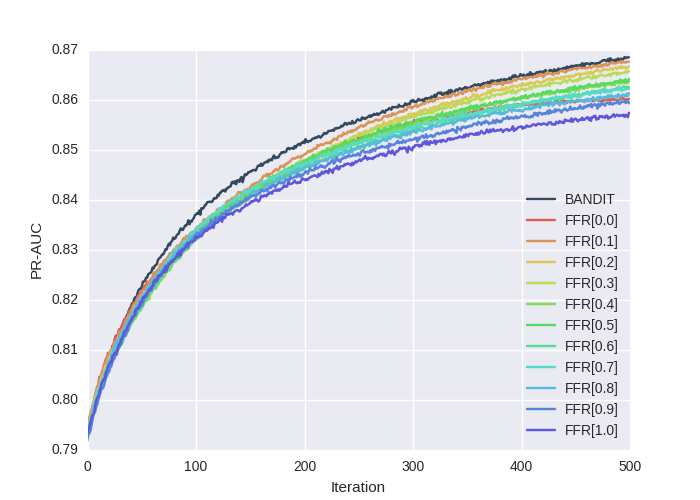
\includegraphics[width=\columnwidth]{fig/interval-mixed-bandit}
		\label{fig:interval-costmixed} 
	}\\
	\subfigure[Document classification experiment]{
    	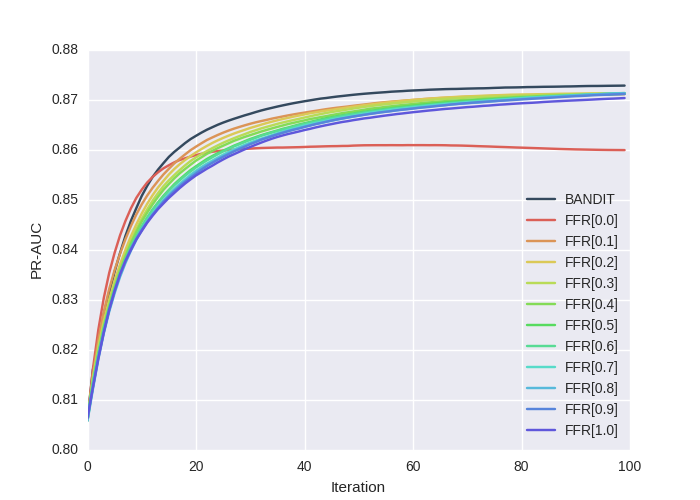
\includegraphics[width=\columnwidth]{fig/RCV1-mixed-bandit}
    	\label{fig:RCV1-costmixed}
    }\\
    \subfigure[Sequence tagging experiment]{
    	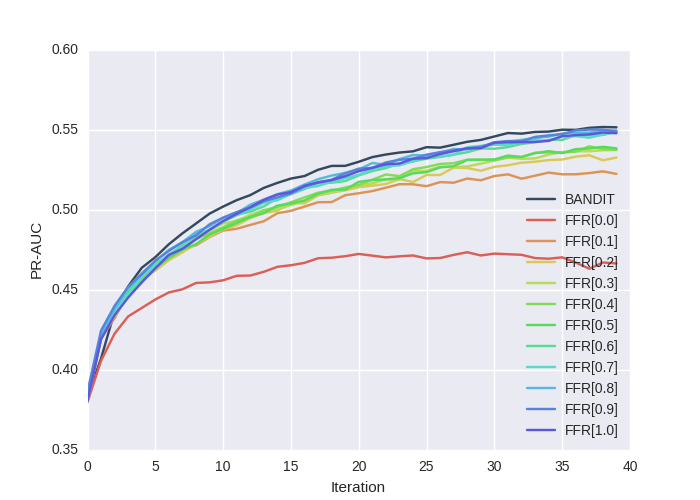
\includegraphics[width=\columnwidth]{fig/richmond-mixed-bandit}
    	\label{fig:richmond-costmixed}
    }
    \caption{Learning curves comparing active FFR and BANDIT method PR-AUC on mixed fine cost}
	\label{fig:costmixed}
\end{figure}



%\input{discussion}


\section{Related Work}
\label{sec:relwork}

To our knowledge, our experiments are the first to demonstrate
how leveraging fine-grained label information can improve the
accuracy of a coarse-grained (root-level) classifier, and the first
investigation into active learning in a hierarchical setting where
label acquisition cost can vary.

Previous work in text classification~\cite{mccallum1998improving} and rich media indexing~\cite{jiang2013} has considered using
hierarchies of labels to improve a fine-grained classifier, through
techniques that back off to coarse
levels of the hierarchy when fine-grained data are sparse. 
By contrast, we present novel techniques
that work in the opposite direction, utilizing selectively
acquired fine-grained labels to improve
classification over coarse categories.
In named entity recognition (NER), some recent work has targeted
fine-grained entity categories~\cite{fleischman2002fine,ling2012fine}
or hierarchies~\cite{yosef2012hyena}.  Our work differs from this
previous work in that we focus on active learning under variable
label acquisition costs.
Our experiments illustrate that our active approach outperforms
passive learning on the NER task, and we demonstrate how the
relative cost of obtaining finer-grained labels impacts
which NER approach is most appropriate to use.

Our approach builds on a variety of previous work in active learning.
We focus on ``pool-based'' active learning, in which
a learner selects instances from a pool of unlabeled data to be 
labeled by an oracle. When acquiring
labels is costly, active learning can reduce
the expense by requesting only a relatively small subset
of the most informative labels~\cite{Rubens2011}.
One criterion used for selection of instances to label is to
choose those that reduce uncertainty. In our case,
uncertainty is measured in terms of the confidence of output values
(e.g., Merialdo~\cite{Merialdo2001}); other measures include
uncertainty in the parameters of probabilistic models~\cite{Hofmann2003}
or the size of a model's decision boundary~\cite{Schohn2000}.  
% Experiments with other active learning approaches in our hierarchical setting is an item of future work.

In previous work, active learning has also been shown 
to reduce sampling bias by utilizing the hierarchical structure of input
features~\cite{Dasgupta2008, Symons2006}. By contrast, 
our work focuses on active learning over hierarchically
structured output labels.

Luo et al.~\cite{lsu-lsal-13} looked at active learning to perform structure
prediction, e.g., to predict a segmentation of an image or a parse tree of a
sentence.  While the predictions their algorithms made are structured in
nature, it is not similar to our work, which predicts labels according to a
fixed hierarchy known {\em a priori} and varying costs.

\section{Conclusions}
\label{sec:concl}

Hierarchical labeling schemes are increasingly common in a variety
of applications.  Our results demonstrate that fine-grained label
data (labels specified at nodes removed from the root of a labeling
tree) can be used to improve precision of a classifier for the
coarse-grained (root) concept.  However, it is likely that such
fine-grained labels will be more expensive to obtain.  We defined
a new active learning approach, {\bf active over-labeling}, to address this scenario, created a family of
hybrid algorithms to actively make label purchase decisions, 
empirically evaluated this family of algorithms, and analyzed the 
relative cost points at which one algorithm is preferred over another
at various budget levels. Finally, we proposed a more sophisticated algorithm
which improves performance by dynamically adjusting the proportion of labels 
purchased at different levels of the labeling tree.

In future work, it would be
interesting to consider other hierarchically labeled data sets with multiple layers, e.g.,
that labeled by the Gene Ontology~\cite{GeneOntology}.


% trigger a \newpage just before the given reference
% number - used to balance the columns on the last page
% adjust value as needed - may need to be readjusted if
% the document is modified later
%\IEEEtriggeratref{8}
% The "triggered" command can be changed if desired:
%\IEEEtriggercmd{\enlargethispage{-5in}}

% references section

% can use a bibliography generated by BibTeX as a .bbl file
% BibTeX documentation can be easily obtained at:
% http://www.ctan.org/tex-archive/biblio/bibtex/contrib/doc/
% The IEEEtran BibTeX style support page is at:
% http://www.michaelshell.org/tex/ieeetran/bibtex/
\bibliographystyle{IEEEtran}
% argument is your BibTeX string definitions and bibliography database(s)
%\bibliography{IEEEabrv,../bib/paper}
%
% <OR> manually copy in the resultant .bbl file
% set second argument of \begin to the number of references
% (used to reserve space for the reference number labels box)


% \bibliography{doug,bib/colt,bib/lrgbrt,bib/textanalysis,bib/me,bib/roc,bib/netw,bib/tutor,bib/extras,bib/active,bib/multi,bib/fuzzy,bib/bio,bib/mcmc,bib/physics,bib/budgeted,bib/bayesnets}


% Generated by IEEEtran.bst, version: 1.13 (2008/09/30)
\begin{small}
\begin{thebibliography}{10}
\providecommand{\url}[1]{#1}
\csname url@samestyle\endcsname
\providecommand{\newblock}{\relax}
\providecommand{\bibinfo}[2]{#2}
\providecommand{\BIBentrySTDinterwordspacing}{\spaceskip=0pt\relax}
\providecommand{\BIBentryALTinterwordstretchfactor}{4}
\providecommand{\BIBentryALTinterwordspacing}{\spaceskip=\fontdimen2\font plus
\BIBentryALTinterwordstretchfactor\fontdimen3\font minus
  \fontdimen4\font\relax}
\providecommand{\BIBforeignlanguage}[2]{{%
\expandafter\ifx\csname l@#1\endcsname\relax
\typeout{** WARNING: IEEEtran.bst: No hyphenation pattern has been}%
\typeout{** loaded for the language `#1'. Using the pattern for}%
\typeout{** the default language instead.}%
\else
\language=\csname l@#1\endcsname
\fi
#2}}
\providecommand{\BIBdecl}{\relax}
\BIBdecl

\bibitem{GeneOntology}
\BIBentryALTinterwordspacing
``The {Gene} {Ontology},'' [Online]. Available:
  \url{geneontology.org}
\BIBentrySTDinterwordspacing

\bibitem{fleischman2002fine}
M.~Fleischman and E.~Hovy, ``Fine-grained classification of named entities,''
  in \emph{Proc. 19th Int. Conf. on Comp.
  Linguistics-Vol 1}, pp. 1--7,  2002. 

\bibitem{ling2012fine}
X.~Ling and D.~S. Weld, ``Fine-grained entity recognition.'' in \emph{AAAI},
  2012.

\bibitem{yosef2012hyena}
M.~A. Yosef, S.~Bauer, J.~Hoffart, M.~Spaniol, and G.~Weikum, ``Hyena:
  Hierarchical type classification for entity names.'' in \emph{COLING
  (Posters)}, 2012, pp. 1361--1370.

\bibitem{finkel2005incorporating}
J.~R. Finkel, T.~Grenager, and C.~Manning, ``Incorporating non-local
  information into information extraction systems by Gibbs sampling,'' 
  \emph{Proc.~of 43rd ACL}, pp. 363--370, 2005.

\bibitem{Lewis2004}
D.~D. Lewis, Y.~Yang, T.~G. Rose, and F.~Li, ``{RCV1: A New Benchmark
  Collection for Text Categorization Research},'' \emph{JMLR},
  vol.~5, pp. 361--397, 2004.

\bibitem{v-tl-84}
L.~G. Valiant, ``A theory of the learnable,'' \emph{Commun. ACM}, vol.~27,
  no.~11, pp. 1134--1142, Nov. 1984.

\bibitem{a-lrsqc-87}
D.~Angluin, ``Learning regular sets from queries and counterexamples,''
  \emph{Inform. Comput.}, vol.~75, pp.~87--106, 1987.

\bibitem{behw-lvd-89}
A.~Blumer, A.~Ehrenfeucht, D.~Haussler, and M.~K. Warmuth, ``Learnability and
  the {V}apnik-{C}hervonenkis dimension,'' \emph{J. ACM}, vol.~36, no.~4, pp.
  929--965, 1989.

\bibitem{m-sncscp-xx}
W.~J. Masek, ``Some {NP}-complete set cover problems,'' unpublished manuscript,
  {MIT} Laboratory for Computer Science.

\bibitem{bb-plapc-03}
N.~Bshouty and L.~Burroughs, ``On the proper learning of axis-parallel
  concepts,'' \emph{JMLR}, vol.~4, pp.~157--176, 2003.

\bibitem{Breiman1996}
L.~Breiman, ``{Stacked regressions},'' \emph{Machine Learning}, vol.~24, pp. 49--64, 1996.

\bibitem{Friedman2001}
J.~H. Friedman, ``{Greedy function approximation: A gradient boosting
  machine},'' \emph{Annals of Statistics}, vol.~29, no.~5, pp. 1189--1232,
  2001.

\bibitem{Auer2002}
P. Auer, N. Cesa-Bianchi, P. Fischer, ``{Finite-time analysis of the multi-armed bandit problem},'' \emph{Machine Learning} 47, 235-256 (2002).

\bibitem{Salton1988}
%\BIBentryALTinterwordspacing
G.~Salton and C.~Buckley, ``{Term-weighting approaches in automatic text
  retrieval},'' \emph{Inf.~Proc.~\&~Man.}, 1988. %[Online].
%  Available:
%  \url{http://www.sciencedirect.com/science/article/pii/0306457388900210}
%\BIBentrySTDinterwordspacing

\bibitem{Cox1958}
D.~Cox, ``{The regression analysis of binary sequences},'' \emph{Jour.~of the
  Royal Stat.~Soc.}, vol.~20, pp.~215--242, 1958.

\bibitem{RichmondDispatch}
%\BIBentryALTinterwordspacing
{University of Richmond Libraries}, ``{\em {Richmond} {Daily} {Dispatch},
  1860--1865},'' 2014. %[Online]. Available:
%  \url{dlxs.richmond.edu/d/ddr/techinfo.html}
%\BIBentrySTDinterwordspacing

\bibitem{Sutton2006}
%\BIBentryALTinterwordspacing
C.~Sutton, ``{An introduction to conditional random fields for relational
  learning},'' \emph{Graphical Models}, vol.~7, p.~93, 2006. %[Online].
%  Available:
%  \url{http://books.google.com/books?hl=en\&amp;lr=\&amp;id=lSkIewOw2WoC\&amp;oi=fnd\&amp;pg=PA93\&amp;dq=An+Introduction+to+Conditional+Random+Fields+for+Relational+Learning\&amp;ots=T-AKP-ger3\&amp;sig=Ew0XSB-xE6hBfQQFdspsv\_qZdcE}
%\BIBentrySTDinterwordspacing

\bibitem{Culotta2004}
%\BIBentryALTinterwordspacing
A.~Culotta, ``{Confidence estimation for information extraction},''
  \emph{HLT-NAACL}, 2004. %[Online]. 
% Available:
%  \url{http://dl.acm.org/citation.cfm?id=1614012}
%\BIBentrySTDinterwordspacing

\bibitem{mccallum1998improving}
A.~McCallum, R.~Rosenfeld, T.~M. Mitchell, and A.~Y. Ng, ``Improving text
  classification by shrinkage in a hierarchy of classes.'' \emph{ICML},
  pp. 359--367, 1998.

\bibitem{Rubens2011}
%\BIBentryALTinterwordspacing
N.~Rubens, D.~Kaplan, and M.~Sugiyama, ``{Active learning in recommender
  systems},'' \emph{Recommender Systems Handbook}, pp. 1--31, 2011. %[Online].
%  Available:
%  \url{http://link.springer.com/chapter/10.1007/978-0-387-85820-3\_23}
%\BIBentrySTDinterwordspacing

\bibitem{Merialdo2001}
%\BIBentryALTinterwordspacing
A.~Merialdo, ``{Improving Collaborative Filtering For New-Users By Smart Object
  Selection},'' \emph{ICMF}, 2001. %[Online]. %Available:
%  \url{http://www.eurecom.fr/publication/670
%  https://www.eurecom.fr/fr/publication/670/download/mm-kohrar-010508.pdf}
%\BIBentrySTDinterwordspacing

\bibitem{Hofmann2003}
%\BIBentryALTinterwordspacing
T.~Hofmann, ``{Collaborative filtering via gaussian probabilistic latent
  semantic analysis},'' in \emph{ SIGIR '03}, p. 259, 2003.
%  \url{http://dl.acm.org/citation.cfm?id=860435.860483}
%\BIBentrySTDinterwordspacing

\bibitem{Schohn2000}
%\BIBentryALTinterwordspacing
G.~Schohn and D.~Cohn, ``{Less is more: Active learning with support vector
  machines},'' \emph{ICML}, pp. 839--846. %, Jun. 2000. %[Online]. %Available:
%  \url{http://dl.acm.org/citation.cfm?id=645529.657802
%  http://citeseerx.ist.psu.edu/viewdoc/download?doi=10.1.1.31.6090\&rep=rep1\&type=pdf}
%\BIBentrySTDinterwordspacing

\bibitem{Dasgupta2008}
%\BIBentryALTinterwordspacing
S.~Dasgupta and D.~Hsu, ``{Hierarchical sampling for active learning},''
  \emph{ICML }, pp. 208--215, 2008. %[Online]. %Available:
%  \url{http://portal.acm.org/citation.cfm?doid=1390156.1390183}
%\BIBentrySTDinterwordspacing

\bibitem{Symons2006}
%\BIBentryALTinterwordspacing
C.~Symons et al.,
  ``{Multi-Criterion Active Learning in Conditional
  Random Fields},'' \emph{ ICTAI}, pp. 323--331, 2006. %[Online].
%  Available:
%  \url{http://ieeexplore.ieee.org/lpdocs/epic03/wrapper.htm?arnumber=4031915
%  http://dl.acm.org/citation.cfm?id=1190614.1191040}
%\BIBentrySTDinterwordspacing

\bibitem{lsu-lsal-13}
W.~Luo, A.~Schwing, and R.~Urtasun, ``Latent structured active learning,'' in
  \emph{NIPS}, 2013.
  
\bibitem{jiang2013}
W.~Jiang and Z.~Ras, ``Multi-label Automatic Indexing of Music by Cascade Classifiers,'' in \emph{Web Intelli. and Agent Sys.}, 2013.

\end{thebibliography}
\end{small}

% that's all folks
\end{document}
